\chapter{مروری بر کارهای گذشته، روش‌ها و ابزارهای موجود}
در این فصل به مرور جامع و شاملی از پژوهش‌های انجام شده در حوزه‌های مرتبط و متداخل با موضوع این پروژه، پرداخته می‌شود. این فصل جزو مهم‌ترین و زمان‌برترین فصل‌های این سند است چرا که تقریبا پیش‌زمینه، استدلال و به نهایت رسیدن این پروژه، در گروه کامل بودن مطالعه و مفصل بودن بررسی‌هایی است که در این فصل انجام می‌شود. ابتدا با مرور و مطالعه بر انواع مدل‌های کیفیتی شروع خواهیم کرد و سپس به مرور روی استفاده‌پذیری در این مدل‌ها تمرکز کرده و سناریوهای سنجش استفاده‌پذیری را مطالعه خواهیم کرد. ده سناریوی بسیار مهم برای مطالعه استفاده‌پذیری کشف شده‌اند که در ادامه فصل به توضیح و شرح آن‌ها و اینکه چگونه می‌توانند در مدل کیفیتی انتخاب شده بگنجند بحث خواهیم نمود. سپس، با یک مطالعه مجلل روی ابزارهای سنجش و آزمون استفاده‌پذیری شاخص، مهم‌ترین ویژگی آن‌ها را استخراج می‌کنیم تا در ادامه بتوانیم بهترین ابزار موجود را پیاده‌سازی کنیم. در انتهای فصل نیز روش‌های کنترل کیفیت داده‌های حاصل از جمع‌سپاری را مورد بحث و بررسی قرار می‌دهیم تا ببینیم کدام یک از روش‌ها برای ابزار ما و هدف نهایی این پروژه، مناسب خواهد بود.
\section{مدل‌های کیفیتی}
با یک نگاه اجمالی بر منابعی همچون
\cite{wagner_software_2013}،
\cite{seffah_usability_2006}، 
\cite{pressman_software_2015}،
\cite{p._miguel_review_2014}
و همچنین
\cite{sommerville_software_2016}
که به بررسی و مقایسه تطبیقی مدل‌های کیفی پرداخته‌اند، به این نکته پی می‌بریم که صحبت از کیفیت و پژوهش در مورد مدل‌های کیفی از همان ابتدا و به صورت همزمان با پژوهش‌های مربوط به توسعه نرم‌افزار و متدولوژی‌ها مورد توجه بوده است.
در شکل
\ref{fig:qmodels}
ملاحظه می‌شود که از سال ۲۰۰۱، به مرور مدل‌های عام‌منظوره‌ای همچون مدل‌های مک‌کال\LTRfootnote{McCall}
و درومی\LTRfootnote{Dromey}
کم‌رنگ‌تر شدند و شاهد معرفی شدن مدل‌های خاص‌منظوره بودیم.
\begin{figure}[H]
	\centering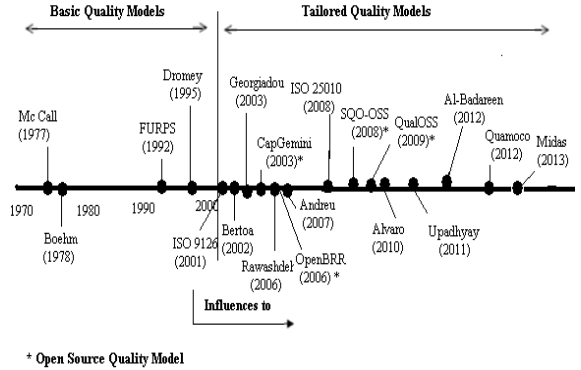
\includegraphics[width=12cm]{Resources/qmodels.PNG}
	\caption[خط زمانی ارائه برخی از مدل‌های کیفیتی]
	{خط زمانی\LTRfootnote{Timeline}
		ارائه برخی از مدل‌های کیفیتی
		\cite{p._miguel_review_2014}؛
		با پیچیده شدن نیازمندی‌ها و گسترش آن‌ها، دسته‌ای از مدل‌ها تحت عنوان مدل‌های کیفیتی
		«\lr{Tailored}»
		در شکل مشخص شده‌اند که به طور خاص و برای یک نیازمندی خاصی ساخته شدند، مدل‌های
		«\lr{Basic}»
		اما به عنوان پایه مدل‌های کیفیتی عمل می‌کند و تقریبا تمامی مدل‌ها از روی این مدل‌های اصلی اقتباس شده‌اند.
	}
	\label{fig:qmodels}
\end{figure}
مدل‌های عام‌منظوره که در شکل با نام «Basic» شناخته می‌شوند، ابعاد کلی کیفیت نرم‌افزار را هدف قرار داده‌اند و تقریبا می‌توانند در هر نرم‌افزاری مورد استفاده قرار بگیرند؛ مدل‌های بعدی که ارائه شدند، روی ابعاد خاصی از سازمان یا محصول نرم‌افزاری تمرکز داشته‌اند. این مدل‌ها در نتیجه افزایش پیچیدگی محصولات نرم‌افزاری و فرایندهای سازمانی، برای استفاده در کاربردهای خاص و برای سازمان‌های خاص توسعه داده شدند
\cite{p._miguel_review_2014}.\\
در بررسی مدل‌های کیفی، مرجع
\cite{wagner_software_2013}
دسته‌بندی‌ای را ارائه داده است که بر اساس آن، مدل‌های کیفی را می‌توان به سه دسته سلسله‌مراتبی، مبتنی بر فرامدل و همچنین مدل‌های ضمنی تقسیم‌بندی کرد که توضیحات هرکدام در ادامه به صورت مختصر قید شده است.
\subsection{مدل‌های سلسله‌مراتبی}
روش‌های بوهیوم\LTRfootnote{Boehm}
\cite{boehm_quantitative_1976}
و مک‌کال
\cite{mccall_factors_1977}
در ارائه مدل کیفی، تشابه زیادی باهم دارند؛ هر دو در خرد کردن مفهوم کیفیت، از یک روش سلسله‌مراتبی استفاده کردند و مطابق شکل
\ref{fig:heir}
کیفیت را به خصیصه‌های مشخصی (که از آن‌ها با نام فاکتورهای کیفیت یاد می‌شود) تقسیم کرده‌اند. این‌گونه مدل‌ها در طول زمان دچار تغییراتی شدند و تفاوت نحوه تقسیم‌بندی آن‌ها، تفاوت مدل‌ها را پدید آورده است.
به تعبیر واگنر
\cite{wagner_software_2013}
رویکرد این نوع مدل‌های کیفی، خرد کردن کیفیت به معیارهای قابل اندازه‌گیری و در نهایت اندازه‌گیری و مقایسه آن‌هاست. همچنین واگنر در بررسی خود، از نقدهایی همچون «مبهم بودن برخی از این تقسیم‌بندی‌ها و شفاف نبودن آن‌ها به طور کامل» یاد می‌کند که از عوامل مهم ناکارآمدی برخی از آن‌هاست؛ همچنین وی در سال ۲۰۱۲ این نکته را متذکر شد که تنها کمتر از ۲۸٪ سازمان‌های فعال در حوزه نرم‌افزار، از مدل‌های استاندارد در تضمین کیفیت فعالیت‌ها و محصولاتشان استفاده می‌کنند و ۷۱٪ این سازمان‌ها، مدل‌های کیفی خود را از روی این مدل‌های کیفی، گلچین کرده و شخصی‌سازی می‌کنند
\cite{wagner_software_2012}.
\begin{figure}
	\centering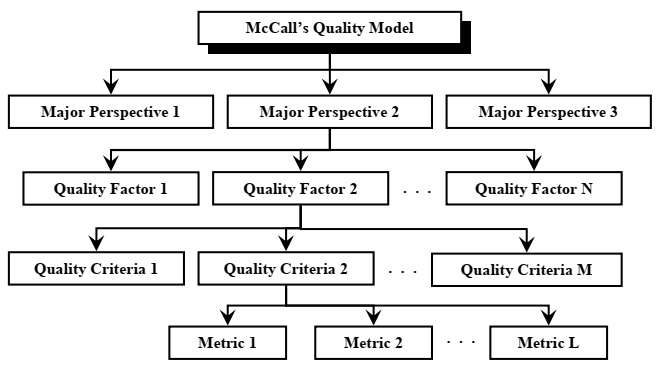
\includegraphics[width=11	cm]{Resources/heir.PNG}
	\caption[ساختار مدل کیفی مک‌کال به عنوان یک مدل کیفی سلسله‌مراتبی]
	{ساختار مدل کیفی مک‌کال به عنوان یک مدل کیفی سلسله‌مراتبی
		\cite{al-qutaish_quality_2010}؛
		این دسته از مدل‌ها کیفیت را به خصیصه‌های خردتری تقسیم می‌کنند و مجددا هر خصیصه را به زیرخصیصه‌های خردتر تقسیم کرده و به همین منوال تا جایی پیش می‌روند که بتوان زیرخصیصه کیفی را به آسانی اندازه‌گیری و شاخصی برای آن تعیین کرد.
	}
	\label{fig:heir}
\end{figure}
همانطور که در شکل
\ref{fig:wagner}
مشاهده می‌شود، طی این بررسی، ۷۹ سازمان مدل‌های کیفیتی شخصی‌سازی‌شده توسط سازمان خود را در اولویت قرار داده و از آن‌ها استفاده می‌کنند. طبق اظهارات این بررسی و همچنین بسیاری از منابع دیگر همچون
\cite{pressman_software_2015} و
\cite{sommerville_software_2016}،
نیاز برای شخصی‌سازی مدل‌های کیفیتی استاندارد وجود دارد. چرا که این مدل‌های سلسله‌مراتبی، به صورت تجریدی بیان شده‌اند و نیازمند دقیق شدن روی خصیصه‌ها و روش‌های اندازه‌گیری هر خصیصه هستند.
\begin{figure}
	\centering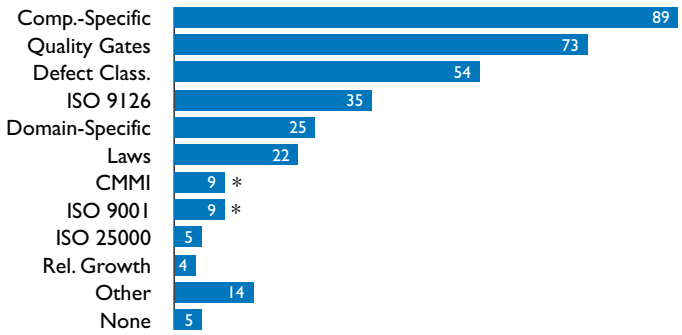
\includegraphics[width=11cm]{Resources/wagner.PNG}
	\caption[بررسی انواع مدل‌ها/رویه‌های کیفیتی استفاده شده در سازمان‌ها]
	{بررسی انواع مدل/رویه‌های کیفیتی استفاده شده در سازمان‌ها
		\cite{wagner_software_2012}؛
		ملاحظه می‌شود که ۸۹ شرکت (تعداد زیادی) فعال در حوزه فناوری اطلاعات در آلمان، به منظور تضمین کیفیت محصولات خود، مدل کیفیتی مختص به خود را توسعه داده‌اند. اما در توسعه این مدل‌ها، همواره مدل‌های اصلی مورد اقتباس واقع شده‌اند و از آن‌ها استفاده شده است.
	}
	\label{fig:wagner}
\end{figure}
\subsection{مدل‌های مبتنی بر فرامدل}
با آشکار شدن این نیاز که می‌بایست مدل‌های پایه‌ای را بیشتر شفاف‌سازی کرد و آن‌ها را بر نیازمندی‌ها تطبیق بیشتری داد، ایده ارائه فرامدل‌ها مطرح شد. فرامدل در اصل مدلی از یک مدل کیفی است؛ قواعد و ساختارهایی که برای توصیف دقیق یک مدل کیفی نیاز داریم (همچون خصیصه‌ها و نحوه اندازه‌گیری آن‌ها)، توسط فرامدل تعیین می‌گردند
\cite{deissenboeck_software_2009}.
به عبارت دیگر، توصیف اینکه چگونه یک مدل کیفی می‌تواند بر نیازمندی‌ها منطبق شود، به عهده فرامدل است
\cite{wagner_software_2013}.
درومی به عنوان مثال، در سال ۱۹۹۵، فرامدل نسبتا مفصلی ارائه داد که ذیل آن، میان مولفه‌های محصول نرم‌افزاری (که باید حامل کیفیت باشند - مانند کد منبع نرم‌افزار) و ویژگی‌های عملیاتی نرم‌افزار تفاوت و تمایز قائل شد
\cite{dromey_model_1995}.
\subsection{مدل‌های آماری و ضمنی}
این مدل‌ها سعی در ترجمه مفهوم اطمینان‌پذیری سخت‌افزار و استفاده آن در حوزه نرم‌افزار را دارند. ایده اصلی استفاده از این مدل‌ها، مشاهده خرابی‌ها در طول زمان و پیش‌بینی روند رخ دادن خرابی‌ها در آینده است. به منظور دستیابی به خصیصه‌های کیفیتی مشخصی که برای نیازهای توسعه محور بیان شده، در برخی از مدل‌ها سعی شده از داده‌های آماری برای به دست آوردن برخی از ویژگی‌ها و خصیصه‌ها استفاده شود.\\
به عنوان مثالی برای این نوع مدل‌ها می‌توان به مدل‌های
\textit{رشد اعتمادپذیری}\LTRfootnote{Reliability Growth Models}
\cite{musa_software_2004}
اشاره کرد. مدل‌هایی که از الگوریتم‌ها و روش‌های یادگیری ماشین برای تخمین موارد مختلف، از قبیل مولفه‌های آسیب‌پذیر و یا غیرکارا و مولفه‌هایی که دارای برخی از ویژگی‌های کیفی خاص نیستند نیز از این نوع‌اند که نمونه‌ای از این مدل‌ها در مرجع
\cite{neuhaus_predicting_2007}
تحت عنوان «وولتور»\LTRfootnote{Vulture}
یاد شده؛ این مدل، از روش‌های یادگیری ماشین و از یک پایگاه دانش آسیب‌پذیری استفاده می‌کند تا در طول زمان و با گسترش نرم‌افزار، بتواند مولفه‌های آسیب‌پذیر نرم‌افزار را پیش‌بینی کند.\\
همچنین به تعبیر مرجع‌های
\cite{sommerville_software_2016}
و
\cite{wagner_software_2013}،
ابزارها و روش‌های مرور، داشبوردهای مدیریتی و مصورسازی داده، ابزارهای شناخت الگوی رخ‌داد خطا در کد منبع نرم‌افزار و چک‌لیست‌ها، که شاید در ظاهر به طور مستقیم ارتباطی با مدل‌های کیفی نداشته باشند، اما در نهایت به یک یا چند خصیصه کیفی در ذیل یک مدل کیفی ختم می‌شوند؛ این اشاره به مدل‌های کیفی به صورت ضمنی و غیرصریح بوده و اغلب به طور دقیق ارتباط خود با مدل‌ها را مشخص نکرده‌اند. در نتیجه‌ی ‌تمام موارد ذکر شده، تضمین و کنترل کیفیت به واسطه این سازوکارهای غیرصریح و مدل‌هایی که به طور ضمنی مطرح هستند، منجر به پیچیدگی بیشتر و سختی کار خواهد شد.

\section{تمرکز بر استفاده‌پذیری در مدل‌های کیفیتی}
در جدول
\ref{tab:models}\RTLfootnote{
	خصیصه‌های ذکر شده در جدول، همگی ترجمه شده عبارات لاتین هستند و در صورت داشتن ابهام در مورد هرکدام می‌توان به
	\hyperref[sec:glossary]{واژه‌نامه}
	رجوع کرد.
}
مقایسه‌ای تطبیقی میان مدل‌های مطرح از سال ۱۹۷۰ تا ۲۰۱۳ انجام شده است که در انجام این مقایسه، به طور خاص، روی خصیصه استفاده‌پذیری این مدل‌ها تمرکز داشتیم. مدل‌های عام‌منظوره در کنار سایر مدل‌ها به مقایسه درآمده‌اند تا خصیصه‌های استفاده‌پذیری در هرکدام از آن‌ها بررسی شود؛ مدل‌های خاص‌منظوره به خاطر نیاز سازمان خاصی به وجود آمده‌اند که مشتریان مخصوص به خود را داشتند که در صورت تعویض محصول و مشتری و استفاده مدل مفروض در یک سازمان دیگر، الزاما به جواب بهینه منتهی نخواهد شد. در حقیقت ویژگی اصلی مدل‌های کیفیتی مبتنی بر فرامدل و دلیل گستردگی آن‌ها، متفاوت بودن نیازهای مشتریان و شرایط سازمان‌هاست
\cite{sommerville_software_2016}.\\
ارائه این مدل‌ها تا سال ۲۰۱۳ یکی از موضوعات پرطرفدار و داغ تحقیقاتی بوده اما به طور تدریجی و از سال ۲۰۱۳، با داشتن مراجعی همچون
\cite{albert_measuring_2013}
می‌توان مطالعه استفاده‌پذیری و رسیدن به یک محصول استفاده‌پذیر را با چک‌لیست‌ها و مطالعات آزمایشگاهی نیز تامین کرد. به خصوص که مرجع
\cite{wagner_software_2012}
از کسب‌وکارهای زیادی نام می‌برد که از هیچ‌کدام از مدل‌های کیفیتی ارائه شده پیشین استفاده نمی‌کنند و از قضا سودآوری زیادی نیز دارند و موفقیت محصولاتشان از سایر رقبا بیشتر است. توجه به این نکته حائز اهمیت است که با ارائه و بحث در مورد خصیصه‌هایی همچون خصیصه‌های مطرح در مرجع
\cite{albert_measuring_2013}
می‌توان انواع مطالعات مطرح در حوزه استفاده‌پذیری را انجام داد و تقریبا سناریویی نخواهد ماند که توسط این خصیصه‌ها مورد پوشش واقع نشوند. بنابراین با توجه به جدول
\ref{tab:models}
می‌توان نتیجه‌گیری کرد که این خصیصه‌ها، به طور خاص برای بررسی، مطالعه و در نهایت بیشینه کردن استفاده‌پذیری رابط‌های کاربری و همچنین تجربه کاربری، کفایت می‌کنند.
\begin{longtable}[c]{|c|C{2.5cm}|C{1.2cm}|C{7cm}|C{1cm}|}
	\caption[مقایسه تطبیقی مدل‌های کیفیتی ارائه شده با تمرکز بر استفاده‌پذیری]
	{مقایسه تطبیقی مدل‌های کیفیتی ارائه شده با تمرکز بر استفاده‌پذیری\RTLfootnote{
			تمامی خصیصه‌های درج شده در جدول ترجمه شده عناوین انگلسی آن‌ها در منابع مختلف هستند؛ در نتیجه ممکن است در ابتدا گیج‌کننده به نظر بیایند. به منظور پی بردن به اصل اصطلاحات به
			\hyperref[sec:glossary]{واژه‌نامه}
			رجوع شود.
	}؛
	مدل‌های کیفیتی بسیاری از سال‌های ۱۹۷۰ تا به امروز ارائه شده‌اند که تعداد اندکی از آن‌ها به عنوان مدل‌های اصلی کیفیتی قلم‌داد می‌شوند و سلسه‌مراتبی هستند. این مدل‌های پایه‌ای، در ادامه به عنوان پایه و اساس برای توسعه مدل‌های کیفیتی دیگر (مبتنی برفرامدل) قرار داده شده‌اند که می‌توان گفت شمار زیادی از مدل‌های ارائه شده از این نوع هستند. بر این اساس، مدل‌هایی که بیشترین ارجاع در سال‌های گذشته به آن‌ها وجود داشته را طی این جدول بررسی کرده‌ایم.
}
	\label{tab:models} \\
	\hline
	\multicolumn{5}{| c |}{مقایسه تطبیقی مدل‌های کیفیتی}\\
	\hline
	ردیف & مدل کیفیتی & سال ارائه & خصیصه‌های استفاده‌پذیری & مرجع \\
	\hline
	\endfirsthead
	
	\hline
	\multicolumn{5}{| c |}{ادامه جدول \ref{tab:models}}\\
	\hline
	ردیف & مدل کیفیتی & سال ارائه & خصیصه‌های استفاده‌پذیری & مرجع \\
	\hline
	\endhead
	\multicolumn{5}{| c |}{ادامه جدول در صفحه بعد...}\\
	\hline
	\endfoot
	
	\hline
	\endlastfoot
	1 & \lr{McCall} & 1970 & عملیاتی بودن، آموزش، ارتباطاتی بودن & \cite{mccall_factors_1977} \\ \hline
	2 & \lr{Boehm} & 1976 & ترابرپذیری، نگهداری‌پذیری & \cite{boehm_quantitative_1976} \\ \hline
	3 & \lr{IEEE 1061} & 1990 & فهم‌پذیری، آسانی یادگیری، ارتباطاتی بودن & \cite{radatz_ieee_1990} \\ \hline
	4 & \lr{Shackel} & 1991 & تاثیرگذاری، یادگیری‌پذیری، انعطاف‌پذیری، نگرش مثبت & \cite{shackel_usability-context_1991} \\ \hline
	5 & \lr{Bevan} & 1991 & گونه محصول، گونه کاربر، راحتی استفاده، قابلیت پذیرش & \cite{bevan_what_1991} \\ \hline
	6 & \lr{FURPS} & 1992 & فاکتورهای انسانی، زیبایی، مستندسازی، مفاد آموزشی & \cite{grady_practical_1992} \\ \hline
	7 & \lr{Nielsen} & 1994 & یادگیری‌پذیری، بهره‌وری، خاطرسپاری‌پذیری، خطا، رضایت & \cite{nielsen_usability_1994} \\ \hline
	8 & \lr{ISO 9126} & 2001 & درک‌پذیری، یادگیری‌پذیری، عملیاتی بودن، جذابیت، قبول استفاده‌پذیری & \cite{organization_iso/iec_1991}  \\ \hline
	9 & \lr{Bertoa} & 2002 & درک‌پذیری، یادگیری‌پذیری، عملیاتی بودن & \cite{bertoa_quality_2002} \\ \hline
	10 & \lr{Georgiadou} & 2003 & پشتیبانی، یادگیری پذیری، به‌روز بودن مستندات، کمک برخط، سازگاری & \cite{georgiadou_gequamogeneric_2003} \\ \hline
	11 & \lr{Abran} & 2003 & بهره‌وری، تاثیرگذاری، رضایت، یادگیری‌پذیری، امنیت & \cite{abran_usability_2003} \\ \hline
	12 & \lr{Bass} & 2003 & اصلاح‌پذیری، مقیاس‌پذیری، قابلیت استفاده مجدد، کارایی، امنیت & \cite{bass_linking_2003} \\ \hline
	13 & \lr{Schneiderman} & 2005 & زمان آموزش، سرعت کارایی، نرخ خطاهای کاربر، بقای کاربران، رضایت منحصر به فرد & \cite{shneiderman_designing_2004}  \\ \hline
	14 & \lr{Rawashdeh} & 2006 & درک‌پذیری، یادگیری‌پذیری، عملیاتی بودن، پیچیدگی & \cite{rawashdeh_new_2006} \\ \hline
	15 & \lr{ISO 25010} & 2008 & تناسب، شناسایی‌پذیری، یادگیری‌پذیری، عملیاتی بودن، جلوگیری از خطای کاربری، زیبایی رابط کاربری، دسترس‌پذیری & \cite{noauthor_iso_nodate}  \\ \hline
	16 & \lr{Alvaro} & 2010 & درک‌پذیری، یادگیری‌پذیری، عملیاتی بودن & \cite{alvaro_quality_2005, alvaro_software_2010} \\ \hline
	17 & \lr{Alonso-Rios} و بقیه & 2010 & دانایی‌پذیری، عملیاتی بودن، بهره‌وری، استحکام، ایمنی، رضایت منحصر به فرد & \cite{alonso-rios_usability:_2009} \\ \hline
	18 & \lr{Dubey} & 2012 & تاثیرگذاری، بهره‌وری، رضایت، یادگیری‌پذیری & \cite{kumardubey_usability_2012} \\ \hline
	19 & \lr{Tullis} & 2013 & موفقیت‌آمیز بودن وظیفه، زمان انجام وظیفه، خطاها، بهره‌وری، یادگیری‌پذیری، خصیصه‌های موردی، خصیصه‌های خوداعلامی، خصیصه‌های فیزیولوژیکی و رفتاری، خصیصه‌های ترکیبی و مقایسه‌ای، خصیصه‌های وبسایت بلادرنگ، الگوهای‌ مرتب‌سازی  & \cite{albert_measuring_2013} \\ \hline
\end{longtable}
شایان ذکر است که در همه مدل‌های ذکر شده، الزاما به استفاده‌پذیری به عنوان یک خصیصه اصلی در محصول اشاره نشده است؛ در بعضی از مدل‌ها همچون
\lr{ISO 25010}
استفاده‌پذیری یکی از سطوح اصلی بوده، در اولین سطح سلسه‌مراتبی مدل قرار داشته و جزئی از محصول نهایی است و در برخی دیگر همچون
\lr{Boehm}،
به طور صریح و مشخص به استفاده‌پذیری اشاره‌ای نشده است اما در فرآیندهای توسعه محصول روی آن توجه زیادی وجود دارد.\\
همچنین از بررسی مدل‌های کیفیتی مختلف که صرفا برای توسعه سامانه‌های مبتنی بر وب این نتیجه برمی‌آید که هر فرامدل می‌بایست در زمینه مربوط به خود مورد استفاده قرار گیرد و نه جای دیگر
\cite{noauthor_measuringu:_2018}.
نتیجه پیشین به این معنی است که در توسعه سامانه‌های مبتنی بر وب، محدوده کاربران، دانش قبلی آن‌ها، تخصص هرکدام، سن و سایر متغیرهای غیرقابل کنترل توسط توسعه‌دهنده نیز در استفاده‌پذیر بودن این سامانه مبتنی بر وب تاثیرگذار است؛ بنابراین در طراحی رابط کاربری هر سامانه مبتنی بر وب، می‌بایست به این نکات نیز توجه داشت و از آخرین توصیه‌های مربوط به توسعه این نوع سامانه‌ها استفاده کرد
\cite{albert_measuring_2013}.
از جمله این توصیه‌ها و پیشنهاد‌های طراحی، توصیه‌های گوگل برای ساخت سامانه‌های کاربردی مبتنی بر وب پیشرو\LTRfootnote{Progressive Web Applications}
\cite{noauthor_progressive_nodate}
است که در سال ۲۰۱۷ مطرح شده و طبق بررسی‌های انجام شده آینده‌ای روشن در انتظار این نوع از سامانه‌های کاربردی است.

\section{مطالعه استفاده‌پذیری و ارزیابی تجربه کاربری}
خصیصه‌هایی که در مطالعه استفاده‌پذیری و به طور خاص هنگام بررسی تجربه کاربری، اندازه‌گیری می‌شوند و مورد سنجش قرار می‌گیرند داده‌هایی را به دست ما می‌دهند که در بررسی و استفاده از این داده‌ها می‌توان دو رویکرد کلی داشت
\cite{albert_measuring_2013}:
ارزیابی خرد و ارزیابی کلان\RTLfootnote{
	در سال ۱۹۸۶ و طی مقاله‌ای با عنوان «نقش ارزیابی مستمر و چرخشی در طراحی سیستم‌ها برای کیفیت»
	\cite{hewett_role_1986}،
	دو اصطلاح برای مطالعه تجربه کاربری و استفاده‌پذیری
«\lr{Formative}»
	و
«\lr{Summative}»
	مورد استفاده قرار گرفتند که هر دو از مفاهیم کلاس درسی برداشت شده‌اند؛ یک ارزیابی مستمر
	(\lr{Formative})
	به معنی پرسیدن سوال در سر کلاس درس توسط معلم بوده و به صورت تدریجی و خرد خرد است؛ در حالی که یک ارزیابی  کلان
	(\lr{Summative})
	بررسی‌ای است که در انتهای هر بازه (مثلا هنگام امتحانات پایان‌ترم) و با برگزاری آزمونی خاص، ارزیابی‌ها انجام می‌شوند. در مقاله ذکر شده همچنین این مورد مطرح می‌شود که که ارزیابی مستمر و خرد برای رسیدن به دقت بالا در برآورد نیازهای مشتری، بهتر است؛ چرا که طبق مدل تشدید خرابی و خطا که پیش‌تر بررسی شد، خرابی‌ها هرچه کمتر بوده و نیازمندی‌های مشتری از همان ابتدا در نظر گرفته شوند و برآورده شوند، کیفیتی بیشتر با صرف هزینه‌ای کمتر خواهیم داشت.
}.\\
\begin{figure}
	\centering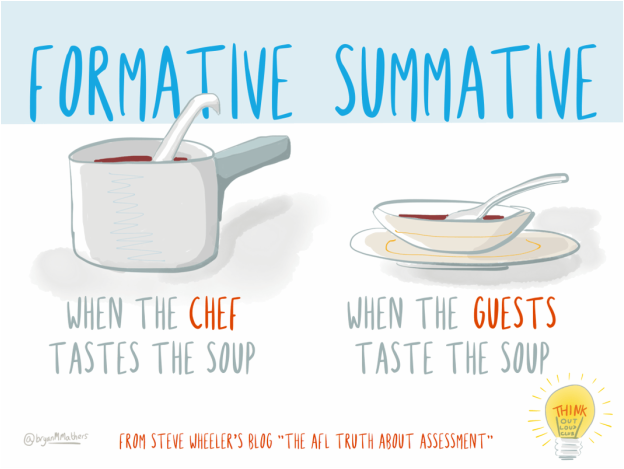
\includegraphics[width=10cm]{Resources/assessment.PNG}
	\caption[مثالی از دو نوع ارزیابی مختلف خرد و کلان]
	{مثالی از دو نوع ارزیابی مختلف خرد و کلان
		\cite{noauthor_formative_nodate}؛
		در این مثال که توسعه‌دهنده نرم‌افزار به آشپز و محصول نهایی به غذای پخته شده توسط آشپز تشبیه شده، تفاوت دو نوع ارزیابی خرد و کلان مطرح شده؛ هنگامی که غذا در حین پخت و توسط آشپز به صورت خرد خرد و در فواصل زمانی کوتاه مورد سنجش قرار می‌گیرد شاهد ارزیابی خرد هستیم و در صورتی که غذا پس از پخت توسط یک منتقد یا مشتری مورد سنجش قرار گیرد، شاهد ارزیابی کلان خواهیم بود.
	}
	\label{fig:assessment}
\end{figure}
همانطور که در شکل
\ref{fig:assessment}
دیده می‌شود، می‌توان این دو نوع ارزیابی را به  چشیدن غذایی بدیل کرد که توسط آشپز و مشتری انجام می‌شوند؛ آشپز در فرآیند پختن غذا به طور مرتب ممکن است غذا را بچشد تا در نهایت خروجی مطلوبی به دست مشتری برسد و غذا از کیفیت لازم برخوردار باشد. در حالی که مشتری در نهایت، محصول نهای را مشاهده می‌کند و صرفا نظر خود در مورد آن غذا و یا کیفیت رستوران را اعلام می‌کند. ذکر این نکته  در همین‌جا خالی از لطف نیست که به وضح می‌توان دریافت که هزینه اعمال تغییرات در صورت درخواست مشتری از آشپز زیاد خواهد بود؛ به طور مشابهی، در صورت عرضه محصول نرم‌افزاری، هزینه تعمیر یک خرابی به مراتب بیشتر از مرور در حین تولید است.
\subsection{ارزیابی خرد}
در یک مطالعه استفاده‌پذیری با رویکرد ارزیابی خرد، محقق به طور مستمر و به صورت دوره‌ای، محصول نهایی را مورد بررسی قرار می‌دهد و در تمامی مراحل تولید نواقص آن را سنجیده و کشف می‌کند و پیشنهاداتی برای رفع آن نواقص ارائه می‌دهد؛ این روند  تا آن جا ادامه پیدا می‌کند که نهایتا یک محصول تقریبا ایده‌آل و یا یک محصول خوب به اندازه کافی\LTRfootnote{
	Good Enough
}
به دست آید. درواقع هدف در این نوع مطالعه هدف بهبود مستمر و رفع ایرادات محصول قبل از عرضه نهایی آن است؛ در نتیجه با بررسی فرآیندهای نرم‌افزاری و همچنین مطالعاتی از قبیل
\cite{sommerville_software_2016}،
\cite{krug_dont_2000} و
\cite{albert_measuring_2013}
به نظر می‌رسد که هرچه ارزیابی خرد زودتر رخ دهد، تاثیر بیشتری روی محصول نهایی و افزایش کیفیت آن خواهد داشت.\\
با اتخاذ این رویکرد، برخی از سوالاتی که می‌توان در فرایند طراحی پرسید عبارتند از:
\begin{itemize}
	\item 
	مهم‌ترین مواردی که کاربران را از رسیدن به اهدافشان منع می‌کند و یا به عدم کارایی آن‌ها می‌شود چیست؟
	\item 
	نقاط قوت و ضعف محصول از نقطه نظر کاربران چیست؟
	\item 
	اشتباهات متداول کاربران هنگام کار با محصول حول چه مواردی است؟
	\item 
	آیا بهبودهای مطرح شده توسط محققین تجربه کاربری، در هر نسخه از طراحی رابط کاربری، مورد استفاده و توجه قرار می‌گیرند؟
	\item 
	پس از عرضه نهایی محصول، چه مواردی در رابطه با استفاده‌پذیری به نظر می‌رسد که هنوز جای کار خواهد داشت؟
	
\end{itemize}
شایان ذکر است که در صورتی که فرصت اصلاح طراحی واسط کاربری وجود نداشته باشد، استفاده از این روش ارزیابی به نظر می‌رسد که کارایی چندانی نداشته باشد و بیشتر باعث هدررفت منابع شود.
\subsection{ارزیابی کلان}
در این روش، محقق همچون یک منتقد، محصول نهایی را از زوایای مختلف مورد بررسی قرار می‌دهد و حتی با محصول‌های دیگر مقایسه می‌کند تا نقدی بر آن وارد سازد. نکته حائز اهمیت این است که در اینجا محصول ارائه شده است و دیگر در فاز توسعه و تولید نیست. هدف از انجام این نوع ارزیابی، پی بردن به این نکته است که این محصول خاص چه‌قدر خوب می‌تواند به نیازمندی‌های کاربران پاسخ دهد و به چه میزان با آن‌ها هم‌جهت است. بر خلاف ارزیابی خرد، این روش، مبتنی بر اصول و قواعد و چک‌لیست‌های مشخصی است که در نهایت محصول با آن‌ها بررسی می‌شود. در مقایسه محصولات مختلف نیز مجددا این اصول و قواعد مبنا قرار می‌گیرند. با بررسی منابع مختلفی از قبیل
\cite{sommerville_software_2016} و
\cite{pressman_software_2015}
می‌توان به این نکته پی برد که سوالاتی از قبیل سوالات زیر بیشتر مناسب انجام این نوع ارزیابی هستند:
\begin{itemize}
	\item 
	آیا اهداف استفاده‌پذیری پروژه (مطرح شده در نیازمندی‌های پروژه) رعایت شده‌اند؟
	\item 
	استفاده‌پذیری کلی سیستم در چه سطحی است؟
	\item 
	نقاط ضعف و قوت محصول مورد نظر در مقایسه با سایر رقبا چیست و چگونه می‌توان در صورت داشتن ضعف، آن را ارتقا داد؟
	\item 
	آیا بهبودهای مطرح برای هر نسخه از نرم‌افزار، پس از عرضه نسخه جدید، اعمال می‌شوند؟
\end{itemize}
در نهایت فراموش نکنیم که همواره تغییر نیازمند صرف هزینه و زمان است؛‌ بنابراین در صورت استفاده از این روش ارزیابی می‌بایست در نظر داشت که برخی فعالیت‌های پسا ارزیابی نیز باید در پس ذهن مدیر پروژه باشد؛ چرا که ممکن است حتی در صورت نیاز پروژه‌ای برای برطرف کردن مشکلات استفاده‌پذیری یک سیستم تعریف شود که خود این پروژه هزینه‌بر باشد.
\subsection{اهداف کاربری}
سوالاتی همچون «آیا محصول مورد نظر نیاز روزانه کاربران را برآورده خواهد کرد و کاربران به طور متداول با این محصول نرم‌افزاری در ارتباط خواهند بود؟» و نیز «آیا کارایی کاربران و بهره‌وری آن‌ها در طول انجام یک وظیفه مشخص در هنگام کار با این نرم‌افزار مهم است؟ چگونه می‌توان آن را بهبود داد؟» به قسمتی از محصول توجه دارند که با نیازمندی‌های کاربر درگیر است. با بررسی‌ مراجعی همچون
\cite{albert_measuring_2013}،
\cite{noauthor_measuringu:_2018}،
\cite{hewett_role_1986} و
\cite{abran_usability_2003}
می‌توان به این نکته پی‌برد که همه این قبیل سوالات که به نیازهای ضمنی و نه الزاما صریح کاربر، در تعامل با رابط کاربری می‌پردازند، به دو خصیصه اساسی و قابل اندازه‌گیری از نیاز کاربران اشاره می‌کنند\RTLfootnote{
	البته باید توجه کرد که کارایی کاربر و رضایت کاربر در اینجا اشاره به دید کاربر به سامانه هدف دارند و نه اینکه خصیصه‌های اصلی مدل کیفیتی باشند. در اینجا کارایی و رضایت از دید کاربر و به عنوان نظر وی در مورد سامانه، مورد نظر هستند.
}: کارایی\LTRfootnote{Performance} و رضایت کاربر\LTRfootnote{Satisfaction}.
\paragraph{کارایی}
به عنوان یک خصیصه کیفیتی به طور خاص در رابطه با تجربه کاربری، به اندازه‌گیری توانایی کاربران در انجام وظایف مشخصی می‌پردازد؛ در این راستا، اندازه‌گیری‌های جنبی نیز اهمیت زیادی پیدا می‌کنند. از جمله این اندازه‌گیری‌ها می‌توان به موارد زیر اشاره کرد که به طور غیر مستقیم در کارایی تاثیرگذار هستند:
\begin{itemize}
	\item 
	زمان سپری شده برای انجام وظیفه
	\item 
	میزان تلاش برای انجام وظیفه (برای مثال تعداد کلیک‌ها و یا توان ذهنی مصرف شده)
	\item 
	زمانی که طول می‌کشد تا کاربر با وظیفه آشنا شود و بدون صرف تلاش خاصی آن را انجام دهد (یادگیری)
\end{itemize}
اندازه‌گیری‌های مربوط به خصیصه کارایی یک رابط کاربری، اهمیت زیادی دارند چرا که اگر کاربران نتوانند وظایف اصلی در رابطه با تعامل با سیستم را به درستی و با موفقیت به انجام برسانند، در عمل محصول نرم‌افزاری به شکست منتهی شده است و یا حداقل رابط کاربری خوبی ندارد و امکان تعامل موفق کاربر وجود نخواهد داشت.
\paragraph{رضایت}
درواقع نظر نهایی کاربر در مورد تعاملش با سیستم است؛ قضاوتی که کاربر در مورد سیستم و نحوه تعاملش با آن می‌کند می‌تواند با جملات مختلفی مانند «استفاده از آن سخت/آسان بود»، «گیج‌کننده/ساده بود» و ... بیان شود. البته که این تعبیرات غیردقیق هستند اما می‌توان با اعطای درجه‌های آزادی خاصی به کاربران، در حین تعامل با سیستم برخی از خصیصه‌ها را از آن‌ها به طور خوداعلامی\LTRfootnote{Self-reported Metrics} از کاربران گزارش عددی گرفت؛ چه بسا که به گفته مراجعی همچون
\cite{albert_measuring_2013}،
\cite{alonso-rios_usability:_2009} و
\cite{seffah_usability_2006}
این خصیصه‌ها در سامانه‌های کاربردی مبتنی بر وب - که هدف اصلی این پروژه هستند - بسیار مهم و تاثیرگذارند. اما باید به این نکته توجه کرد که در محدوده سامانه‌های مبتنی بر وب، رضایت کاربر الزاما همیشه همراه با کارایی حداکثری وی در تعامل با سامانه نیست؛ فاکتورهای بسیاری از قبیل زیبایی و وجود تکنولوژی‌های مختلف، بر این رضایت تاثیر مستقیم دارند و چه بسا که کاربری با رضایت حداکثری از یک سامانه استفاده کند ولی کارایی عملیات وی بسیار پایین باشد.\\
ویژگی‌های محصولی که کاربر با آن در تعامل است به عنوان یکی از اصلی‌ترین مدخل‌ها به بحث رضایت کاربری اهمیت دارند. در درجه دوم اما، کیفیت تعامل به عوامل دیگری همچون دانش قبلی کاربر و سن و جنسیت و غیره وابسته است. در ادامه مدلی برای تشخیص دادن ویژگی‌های محصول نهایی و اینکه کدام یک از آن‌ها و در چه شرایطی منجر به رضایت کاربری خواهند شد معرفی می‌شود.
\paragraph{مدل کانو}
که در سال ۱۹۸۴ و توسط آقای کانو
\cite{kano_attractive_1984}
برای تشخیص دادن ویژگی‌های اشتیاق‌برانگیز و صریح و همچنین ویژگی‌های ضمنی و بایدی یک محصول و همچنین درک تفاوت‌های آن‌ها، ارائه شد. طی این مدل، کیفیت محصول نهایی در گرو پنج دسته از نیازمندی‌های زیر است که رسیدن به هر دسته از این‌ها نیازمند اتخاذ سیاست‌های مختلف در طول ساخت محصول است:
\begin{figure}[H]
	\centering
	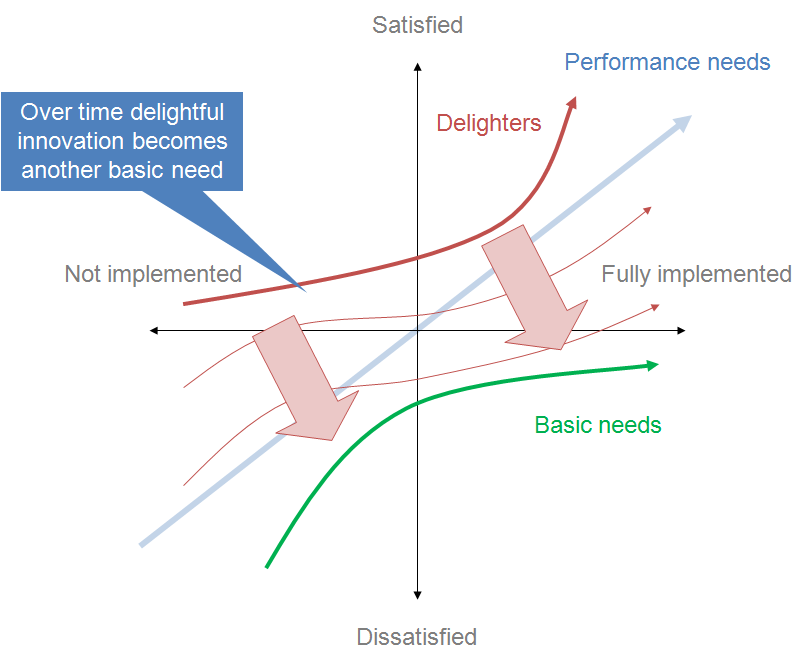
\includegraphics[width=13cm]{Resources/kano_model.PNG}
	\caption[تعبیری از مدل کانو]	{
		تعبیری از مدل کانو
		\cite{noauthor_kano_2018}
	}
	\label{fig:kano}
\end{figure}
\begin{itemize}
	\item 
	نیازمندی‌های بایدی: که مشتریان به طور ضمنی خواستار آن‌ها هستند و ممکن است صریحا بیان نشوند. به عنوان مثال اینکه یک سامانه کاربردی مبتنی بر وب همیشه با یک آدرس اینترنتی خاص
«\lr{URL}»
	در دسترس باشد.
	\item
	نیازمندی‌های تک‌بعدی: که در صورت وجودشان کاربر احساس رضایتمندی و در صورت عدم وجودشان در محصول نهایی، کاربر احساس عدم رضایت از محصول را خواهد داشت. برای نمونه می‌توان به واکنش‌گرا بودن یک سامانه مبتنی بر وب روی پلتفرم موبایل اشاره کرد؛ که گفتنی است این روزها به یکی از ویژگی‌های اصلی موفقیت بسیاری از کسب‌وکارهای فعال در ایران تبدیل شده است.
	\item 
	نیازمندی‌های اشتیاق‌برانگیز: که در صورتی که به طور کامل پیاده‌سازی شوند، منجر به رضایتمندی کاربران خواهند شد ولی در صورت عدم پیاده‌سازی، رضایت کاربران از بین نخواهد رفت. به عنوان مثال اینکه یک سامانه پست الکترونیکی مبتنی بر وب\LTRfootnote{Webmail} در کنار لیست ایمیل‌های دریافتی، وضعیت آب‌وهوا و زمان فعلی و گزیده‌ای از اخبار را نشان دهد می‌تواند یک ویژگی اشتیاق برانگیز باشد.
	\item 
	نیازمندی‌های بی‌تفاوت: بودن و نبودنشان تفاوتی در رضایت مشتری نخواهد کرد. به عنوان مثال در بسیاری از پروژه‌های منتهی به یک سامانه کاربردی مبتنی بر وب، پلتفرم و زبان مورد استفاده برای توسعه سامانه، تفاوتی در رضایت مشتریان ایجاد نخواهد کرد.
	\item 
	نیازمندی‌های معکوس: به دسته‌ای از نیازمندی‌ها اشاره دارد که پرداختن بیش‌ازحد به آن‌ها باعث کاهش رضایت کاربران می‌شود. به عنوان مثال برخی از کاربران ممکن است از ابزارهایی که امکانات زیادی به آن‌ها در داشبورد مدیریتی می‌دهند خوششان بیاید و در مقابل برخی از کاربران از پیچیدگی بیش از حد ابزار گلایه کنند.
\end{itemize}
در شکل
\ref{fig:kano}
ملاحظه می‌شود که بسیاری از ویژگی‌های جذاب محصول که هنوز به عنوان نیازمندی مطرح هستند و هنوز پیاده‌سازی نشده‌اند و درنتجیه کاربر امکان انجام عملیات مورد نظر خود را ندارد، انگیزه‌ای برای ساخت سامانه هستند و پس از اینکه این ویژگی‌های عملیاتی (منحی قرمز رنگ) در محصول پدیدار می‌شوند، رضایت کاربران از محصول افزایش پیدا می‌کند؛ گرچه الزاما شاید این ویژگی‌ها، کارایی بالایی از دید کاربران نداشته باشند. به مرور زمان که فناوری پیشرفت می‌کند، نیازمندی‌های فعلی آهسته آهسته به باید‌های سامانه تبدیل می‌شوند (منحنی سبز رنگ).\\
همچنین در مرجع
\cite{sauerwein_kano_1996}
از خط آبی قابل مشاهده در شکل
\ref{fig:kano}،
به عنوان نیازمندی‌های تک‌بعدی یاد شده است که مشتری فقط به طور صریح و مشخص، این دسته از نیازمندی‌ها را مطرح می‌کند و بقیه نیازمندی‌ها معمولا به طور ضمنی مطرح می‌شوند؛ در نتیجه نقش تجربه در مهندسی نرم‌افزار و تولید سیستم‌های باکیفیت را می‌توان کمابیش مشاهده کرد؛ هرچه دانش بیشتری به بدیهیات و سهل‌های ممتنع موجود در نیازمندی‌ها داشته باشیم و اظهارمندی نیازمندی شفاف و مدون‌تری در دست باشد، محصول نهایی با کیفیت‌تر و هزینه و وقت صرف شده کم‌تر خواهد بود.\\
\begin{figure}[H]
	\centering
	\subfloat[تاثیر نیازمندی‌های اشتیاق‌بر‌انگیز]{
		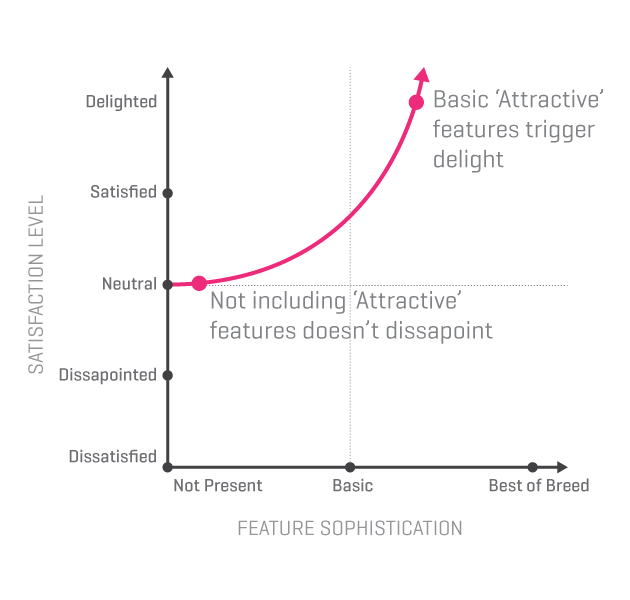
\includegraphics[width=5.5cm]{Resources/kano_attractive.PNG}
	}
	\subfloat[تاثیر نیازمندی‌های تک‌بعدی]{
		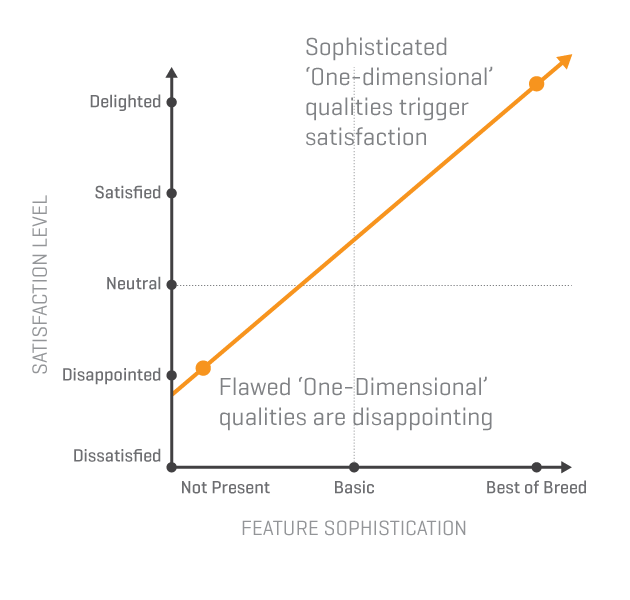
\includegraphics[width=5.5cm]{Resources/kano_one.PNG}
	}
	\hspace{0mm}
	\subfloat[تاثیر نیازمندی‌های بایدی]{
		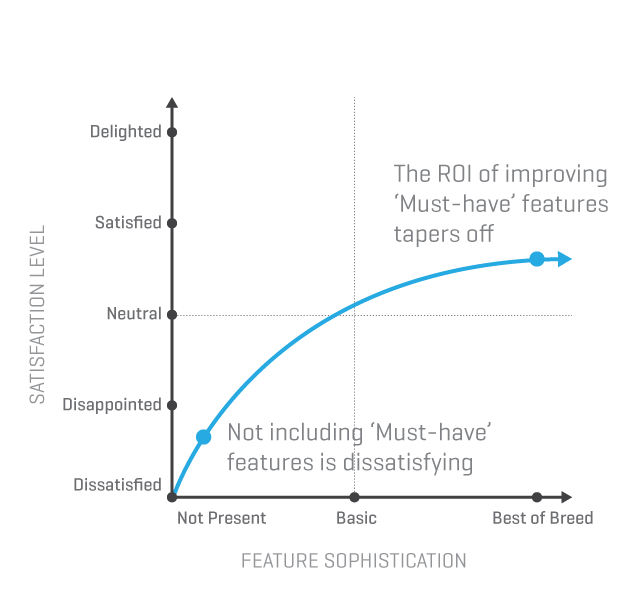
\includegraphics[width=5.5cm]{Resources/kano_must.PNG}
	}
	\subfloat[تاثیر نیازمندی‌های بی‌تفاوت]{
		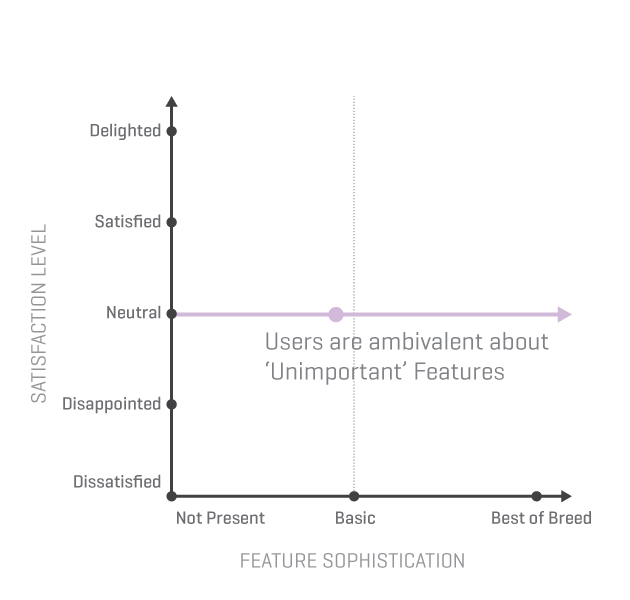
\includegraphics[width=5.5cm]{Resources/kano_unimportant.PNG}
	}
	\hspace{0mm}
	\subfloat[تاثیر نیازمندی‌های معکوس]{
		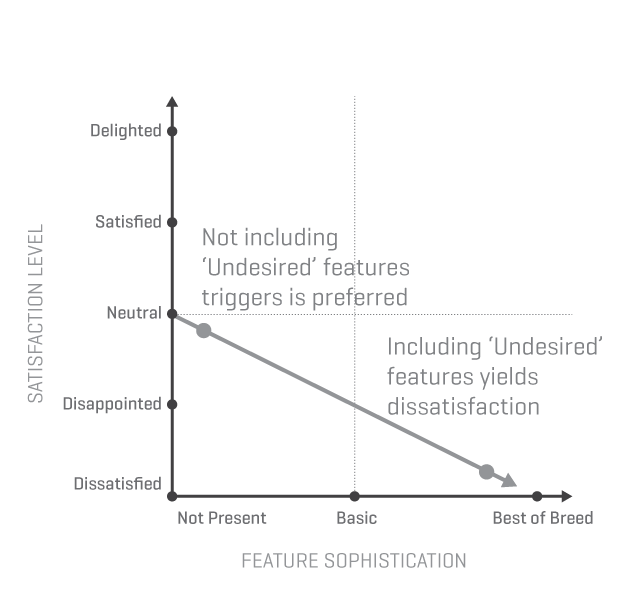
\includegraphics[width=5.5cm]{Resources/kano_undesired.PNG}
	}
	\subfloat[تجمیع نیازمندی‌ها و تاثیرگذاری آن‌ها روی رضایت مشتریان]{
		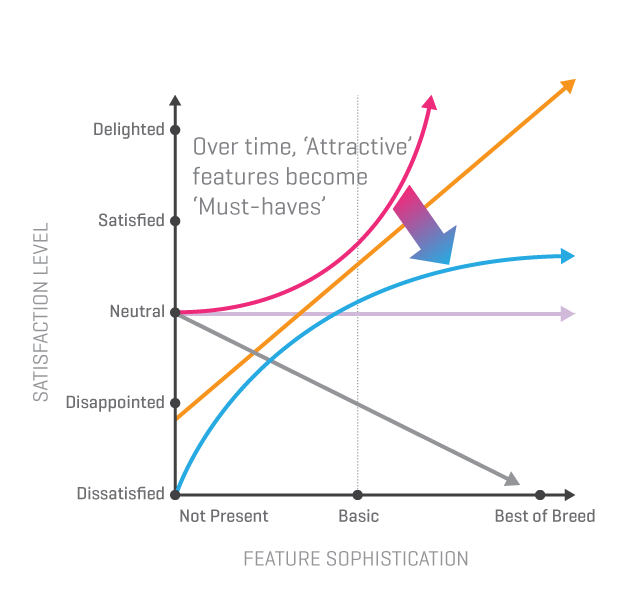
\includegraphics[width=5.5cm]{Resources/kano_model2.PNG}
	}
	\caption[تفسیری از مدل کانو؛ ارتباط رضایت کاربر و ویژگی‌های محصول]
	{تفسیری از مدل کانو؛ ارتباط رضایت کاربر و ویژگی‌های محصول
		\cite{noauthor_leveraging_2012}؛
		نیازمندی‌های اشتیاق‌برانگیز کاربر، خواسته کاربران نیست ولی در صورت پیاده‌سازی موفق، موج بزرگی از رضایت را در بر خواهد داشت (آ). نیازمندی‌های تک‌بعدی در صورت عدم پیاده‌سازی، موجب نارضایتی خواهد بود (ب). نیازمندی‌های بایدی که درواقع خواسته اصلی کاربران بوده و باید به طور کامل پیاده‌سازی شوند تا رضایت حداقلی کسب شود (ج). نیازمندی‌های بی‌تفاوت نیز بود و نبودشان در محصول نهایی تفاوتی در رضایت مشتری ایجاد نخواهد کرد (د). نیازمندی‌های معکوس نشان داده‌اند که هرچه بیشتر به آن‌ها پرداخته شود، باعث بروز نارضایتی بیشتری خواهند شد (ه). در واقع هر ویژگی‌ای از محصول نهایی، مادامی که پیاده‌سازی نشده است، دچار انگیزش کاربر می‌شود. نیازمندی‌های تک بعدی پس از اینکه به کاملی پیاده‌سازی شد و کاربر از آن استفاده کرد، دچار افزایش رضایت‌مندی کاربر شده و در نهایت و پس از گذشت اندک زمانی، این ویژگی به یک ویژگی بایدی تبدیل می‌شود که کاربر حتی شاید به طور صریح به آن اشاره نکند ولی نبود آن در محصول باعث عدم رضایتمندی خواهد شد (و).
	}
	\label{fig:kano2}
\end{figure}
تعاریف انواع نیازمندی‌های مطرح شده توسط کانو به جهت اهمیتی که در شناخت خصیصه‌های کیفیتی این پروژه دارند، بار دیگر در شکل
\ref{fig:kano2}
ذکر شده است. مطابق این شکل، ممکن است با برهم زدن معاملات و همواره با تحویل دادن نیاز‌مندی‌های شگفت‌انگیز، مشتریان خود را غافل‌گیر کنیم و برای کسب رضایت موقتی، آن‌ها را از نیازمندی‌های اصلی دور کنیم، اما باید همواره در خاطر داشت که این استراتژی محکوم به شکست است چرا که محلول زمان در نهایت اشتیاق کاربران را در خود حل کرده و غافل‌گیری‌های دیروز تبدیل به باید‌های امروز خواهند بود و دیگر نمی‌توان ارزش افزوده‌ای نسبت به سایر رقیبان و یا نسبت به وضعیت دیروز سازمان خودمان، ارائه داد.\\
نتیجه نهایی از دو بحث پیشین در مورد رضایت کاربر از سامانه و کارایی\LTRfootnote{Performance} کاربر در تعامل با سامانه، این که، این دو خصیصه الزاما دارای همبستگی خاصی نیستند؛ ولی همواره باید در اندازه‌گیری استفاده‌پذیری مدنظر قرار بگیرند چرا که طبق تعریف استفاده‌پذیری، در یک سیستم استفاده‌پذیر، کاربر می‌بایست در نهایت از سیستم راضی بوده باشد و تجربه کاربری خوبی (کارایی در هنگام استفاده از محصول) داشته باشد.
\section{سناریو‌های سنجش استفاده‌پذیری و خصیصه‌های هرکدام}
با مقایسه تطبیقی انجام شده در جدول
\ref{tab:models}
در رابطه با مدل‌های کیفیتی مختلف و همچنین با بررسی مراجعی همچون
\cite{wagner_software_2012}،
\cite{wagner_software_2013} و
\cite{albert_measuring_2013}
می‌توان نتیجه گرفت که در زمان انتخاب خصیصه‌های اندازه‌گیری استفاده‌پذیری در یک محصول (و نه الزاما یک محصول نرم‌افزاری)، می‌بایست به نکاتی از قبیل اهداف مطالعه استفاده‌پذیری\RTLfootnote{اینکه برای ارتقای محصول نهایی و ساخت یک نسخه دیگر است یا برای پیشگیری از بروز خرابی‌های بعدی و ...}، اهداف کاربری محصول\RTLfootnote{اینکه کاربر چه هدفی را از استفاده کردن از این محصول دنبال می‌کند}، فناوری‌ها و ابزارهای موجود برای جمع‌آوری داده و همچنین بودجه و زمان موجود برای تحقیق درباره استفاده‌پذیری، می‌بایست توجه کرد.\\
به تعبیر مرجع
\cite{albert_measuring_2013}،
در دنیای کنونی که نیازمندی‌ها بسیار گسترده و مفصل شده‌اند و جزئی‌ترین تغییرات در نیازمندی‌های مشتری ممکن است دامنه و حوزه مخاطبان یک سامانه را عوض کند و همچنین از آن‌جایی که در هر مطالعه استفاده‌پذیری، ویژگی‌ها و خصیصه‌های خاص آن مطالعه مدنظر قرار می‌گیرند -که الزاما با اهداف سایر مطالعات استفاده‌پذیری یکسان نیستند- نمی‌توان مجموعه‌ای از خصیصه‌های مشخص و شسته‌رفته‌ای برای اندازه‌گیری و سنجش استفاده‌پذیری در تمام سامانه‌های کاربردی مبتنی بر وب ارائه داد؛‌
در حقیقت، طبق ادعای مرجع
\cite{wagner_software_2012}
بیش از ۷۰٪ سازمان‌های فعال در حوزه فناوری اطلاعات، به منظور تامین و تضمین کیفیت در محصولات نرم‌افزاری خود، مدل‌های گلچین شده و سفارشی‌سازی شده خود را استفاده می‌کنند. بنابراین این پندار که برای تمامی سامانه‌های مبتنی بر وب می‌توان یک مدل کیفیتی ثابت ارائه کرد، غیرمنطقی به نظر می‌رسد. در عوض می‌توان با بررسی سرگذشت تاریخی مدل‌های کیفی و از طریق مقایسه تطبیقی آن‌ها در جدول
\ref{tab:models}
و نیز مطالعه مراجع مختلفی همچون
\cite{alonso-rios_usability:_2009}،
\cite{bass_linking_2003}،
\cite{bevan_what_1991}،
\cite{pressman_software_2015}،
\cite{sommerville_software_2016}
و
\cite{albert_measuring_2013}
که در زمینه تجربه کاربری و استفاده‌پذیری نتایج تحقیقات ارزشمندی را ارائه کرده‌اند، به این نتیجه دست یافت که دسته‌بندی‌های کلی‌ای از انواع مطالعات استفاده‌پذیری می‌توان ارائه نمود، که در هر دسته، با توجه به اهداف و نتایج مورد نیاز مطالعه، خصیصه‌های خاصی اهمیت بیشتری پیدا می‌کنند و می‌توان به آن‌ها پرداخت.\\
یکی از انواع فرامدل‌ها که بر مبنای مدل‌های سلسه‌مراتبی و به طور خاص برای استفاده‌پذیری سامانه‌های کاربردی مبتنی بر وب ساخته شده است در مرجع
\cite{albert_measuring_2013}
ذکر شده است\RTLfootnote{
	البته تمامی خصیصه‌های مطرح برای استفاده‌پذیری در این مدل به طور کامل شرح و بسط داده نشده‌اند؛ چرا که به گفته ارائه دهنده، بسیاری از اقدامات به زمینه مورد مطالعه و تست وابسته بوده و در نتیجه مشخص کردن جزییات نهایی با تیم تضمین کیفیت (تست و ارزیابی استفاده‌پذیری) است. همچنین شایان ذکر است که هیچگاه منبع ذکر شده از خصیصه‌هایی که عنوان کرده به عنوان یک چارچوب و یا فرامدل یاد نکرده است؛ اما به جهت اهمیت استدلال و بررسی‌های این منبع و همچنین ارجاعات زیاد به آن، چه در صنعت و ابزارهایی همچون
	\lr{CrazyEgg}
	و چه در دنیای تحقیقات، اهمیت این خصیصه‌های کیفیتی را به عنوان یک فرامدل کیفیتی دو چندان می‌کند.
}.
با بررسی‌های انجام گرفته روی انواع مدل‌های کیفیتی عام و خاص منظوره که در موقعیت‌های مختلف ارائه شده‌اند، ده سناریوی مهم برای مطالعه استفاده‌پذیری در وب‌اپلیکیشن‌ها مطرح هستند؛ که می‌توان عناوین هرکدام و خصیصه‌های مناسب هر سناریو را در جدول
\ref{tab:10usability}
مشاهده کرد. در ادامه به بررسی هرکدام از این ده سناریو می‌پردازیم.
\begin{table}
	\caption[سناریوهای متداول مطالعه استفاده‌پذیری و خصیصه‌هایی که می‌توان در نظر گرفت]{
		سناریوهای متداول مطالعه استفاده‌پذیری و خصیصه‌هایی که می‌توان در نظر گرفت
		\cite{albert_measuring_2013}؛
		این سناریو‌ها هر کدام از دیدی خاص به استفاده‌پذیری تاکید داشته و روی آن تمرکز می‌کنند. ممکن است در یک سناریو تعداد بسیاری از خصیصه‌های کیفیتی را بتوان اندازه‌گیری و سنجش کرد ولی در دیگری تعداد بسیار کمی را، اما به تعبیر مرجع ذکر شده، این امر روی محبوبیت هیچ‌کدام از سناریوها تاثیری نگذاشته.
	}
	\label{tab:10usability}
	\centering
	%	\resizebox{\textwidth}{!}{%
	\begin{tabular}{|C{5cm}|c|c|c|c|c|c|c|c|c|c|c|}
		\hline
		‏هدف و سناریوی مطالعه استفاده‌پذیری
		& 
		\rotatebox{90}{‏موفقیت‌آمیز بودن وظیفه}
		& 
		\rotatebox{90}{زمان انجام وظیفه}
		& 
		\rotatebox{90}{خطاها}
		& 
		\rotatebox{90}{بهره‌وری}
		& 
		\rotatebox{90}{یادگیری‌ پذیری}
		& 
		\rotatebox{90}{خصیصه‌های موردی}
		& 
		\rotatebox{90}{خصیصه‌های خوداعلامی}
		& 
		\rotatebox{90}{خصیصه‌های فیزیولوژیکی و رفتاری}
		& 
		\rotatebox{90}{خصیصه‌های ترکیبی و مقایسه‌ای}
		& 
		\rotatebox{90}{خصیصه‌های وبسایت بلادرنگ}
		& 
		\rotatebox{90}{الگوهای‌ مرتب‌سازی}
		\\ \hline
		انجام یک تراکنش & × &  &  & × &  & × & × &  &  & × &  \\ \hline
		مقایسه محصولات & × &  &  & × &  &  & × &  & × &  &  \\ \hline
		ارزیابی استفاده مکرر از محصول & × & × &  & × & × &  & × &  &  &  &  \\ \hline
		ارزیابی پیمایش و معماری اطلاعات سامانه & × &  & × & × &  &  &  &  &  &  & × \\ \hline
		افزایش آگاهی &  &  &  &  &  &  & × & × &  & × &  \\ \hline
		کشف مشکل &  &  &  &  &  & × & × &  &  &  &  \\ \hline
		حداکثرسازی استفاده‌پذیری یک محصول حیاتی & × &  & × & × &  &  &  &  &  &  &  \\ \hline
		ایجاد تجربه کاربری مثبت &  &  &  &  &  &  & × & × &  &  &  \\ \hline
		ارزیابی تاثیرات تغییرات جزئی و نامحسوس &  &  &  &  &  &  &  &  &  & × &  \\ \hline
		مقایسه طراحی‌های مختلف & × & × &  &  &  & × & × &  & × &  &  \\ \hline
	\end{tabular}%
	%	}
\end{table}
نکته قابل تامل و مهم این است که در هر کدام از این ده سناریوی مطرح شده، الزاما به تمام ابعاد کیفیتی نگاه نمی‌شود؛ هرچیزی که باعث می‌شود استفاده‌پذیری تحت‌تاثیر قرار بگیرد اهمیت داشته و به جز آن بررسی نمی‌شود. حتی ممکن است در یک سناریو، مواردی از قبیل طراحی پیمایش و طراحی مولفه (رجوع شود به هرم طراحی سامانه‌های کاربردی مبتنی بر وب، شکل \ref{fig:pyramid}) نیز مورد بحث و بررسی قرار گیرند. در ادامه به بررسی هرکدام از سناریوهای ذکر شده در جدول
\ref{tab:10usability}
پرداخته شده و پس از آن توضیح هر خصیصه ذکر شده است.
\subsection{سناریو‌های مطرح در مطالعه استفاده‌پذیری}
\subsubsection{انجام یک تراکنش}
برخی از مطالعات استفاده‌پذیری به جهت افزایش بهره‌وری بیشتر، بهبود و هموارتر شدن روند انجام یک تراکنش هستند؛ این تراکنش می‌تواند «تغییر گذرواژه»، «انجام یک خرید» و یا هر فرایند دیگری باشد. اساسا یک تراکنش دارای یک نقطه آغاز و یک نقطه پایان مشخص و واضح است؛ مثلا در یک سایت خرید و فروش برخط کالا، قرار دادن یک قلم کالا در سبد خرید و اتمام خرید و تایید شدن سفارش، به ترتیب، نقاط شروع و پایان تراکنش هستند.
\subsubsection{مقایسه محصولات}
هدف از برخی مطالعات استفاده‌پذیری، مقایسه بین یک نسخه از یک محصول و یک نسخه از محصول دیگر و یا نسخه‌های قبلی همان محصول، به منظور یافتن نقاط ضعف و قوت هر کدام در طراحی و استفاده‌پذیری است. بنابراین می‌توان گفت که با مقیاسه محصولات می‌توان ارزیابی خوبی از استفاده‌پذیری سامانه هدف، در مقایسه با رقبا داشت و پتانسیل‌های موجود برای افزایش استفاده‌پذیری را شناخت. البته که در این مقایسه می‌بایست امتیازدهی به خصیصه‌های مختلف انجام شود و سپس برترین گزینه انتخاب شود؛ اما انتخاب خصیصه‌ها به این آسانی‌ها هم نیست، چرا که به کاربرد و محدوده سامانه هدف بسیار وابسته‌ است. برخی از سامانه‌ها به منظور افزایش بهره‌وری کاربران ساخته شده‌اند در حالی که برخی دیگر فقط روی تجربه‌کاربری مثبت تمرکز کرده‌اند.
\subsubsection{ارزیابی استفاده مکرر از محصول}
بسیاری از محصولات و سامانه‌های نرم‌افزاری از جمله وب‌سایت‌های شبکه‌های اجتماعی، سامانه‌های اتوماسیون و ... برای استفاده مکرر در طول روز ساخته شده‌اند و برای رسیدن به همین هدف می‌بایست هم استفاده از آن‌ها آسان باشد و هم بهره‌وری زیادی داشته باشند؛ بنابراین در این سناریوی بررسی و با شمردن اهداف پیشین، به نظر می‌رسد که زمان صرف شده برای انجام یک وظیفه از جمله مهم‌ترین خصیصه‌ها برای اندازه‌گیری استفاده‌پذیری به شمار می‌آید.
\subsubsection{ارزیابی پیمایش و معماری اطلاعات سامانه}
به تعبیر مرجع
\cite{albert_measuring_2013}
این سناریو معروف‌ترین سناریو برای سنجش استفاده‌پذیری سامانه‌های مبتنی بر وب است. در انجام مطالعه استفاده‌پذیری طبق این سناریو، می‌توان مواردی همچون «اطمینان از اینکه کاربران حتما چیزی را که می‌خواهند پیدا می‌کنند»، «در صفحات مختلف به آسانی پیمایش می‌کنند» و مواردی از این دست را نیز جزوی از اهداف مطالعه دانست. به طور معمول این مطالعات شامل طرح‌های مفهومی قبل از پیاده‌سازی هستند که هدف اصلی در این پروژه نیز بررسی و سنجش استفاده‌پذیری این طرح‌های مفهومی است؛ درواقع در این طرح‌های مفهومی نحوه بدست آوردن اطلاعات و طراحی پیمایش و تجربه ابتدایی کاربری به قدری مهم است که باید قبل از هر چیزی، و در اولین وهله، تعیین تکلیف شوند.
از جمله خصیصه‌های مهم در این سناریو، موفقیت انجام وظیفه‌های مختلف است.
\subsubsection{افزایش آگاهی}
گاهی اوقات تغییرات در رابط‌های کاربری، فقط به جهت افزایش بهره‌وری کاربر نیست؛ بلکه هدف از اعمال تغییرات در سامانه، افزایش آگاهی نسبت به یک قسمت خاص است. این مسئله در مورد تبلیغات برخط درست است؛ علاوه بر آن، در مواردی هم که پتانسیل‌های کارکردی یک سامانه، به تمامی مورد استفاده قرار نمی‌گیرند نیز این مسئله صادق است.
\subsubsection{کشف مشکل}
در این نوع مطالعه هدف پیدا کردن مشکلات عمده در استفاده‌پذیری محصول است. گاهی اوقات به دلایل مختلفی از جمله سهل ممتنع بودن و یا مخفی بودن مشکلات استفاده‌پذیری در چشم توسعه‌دهنده، عملا تیم توسعه و تولید محصول قادر به کشف مشکلات استفاده‌پذیری محصول نیستند، در حالی که مشتریان از این نوع مشکلات گلایه می‌کنند. معمولا این نوع مطالعه‌ها انتهای باز دارند و نتیجه‌گیری قاطعی نمی‌شود از آن‌ها کرد.
\subsubsection{حداکثرسازی استفاده‌پذیری یک محصول حیاتی}
اگرچه تولیدکنندگان بررخی از محصولات و سامانه‌ها، همچون شبکه‌های اجتماعی، وبلاگ‌ها و ... به دنبال آسان کردن هرچه بیشتر نحوه تعامل کاربران و راحتی کار آن‌ها هستند، برخی از محصولات و سامانه‌های حساس
\emph{باید}
استفاده‌پذیری بالا و راحتی استفاده داشته باشند. از جمله این سامانه‌ها می‌توان به سامانه‌های رای‌گیری، سامانه‌های خروج اضطراری هواپیماها و ... اشاره کرد. فلسفه وجودی سامانه‌های حساس، همچون سایر سامانه‌ها، این است که کاربر می‌بایست در مجموع چند کار بسیار محدود را با آن‌ها انجام دهد. اما تفاوت آن‌ها با سامانه‌های عادی در این است که کاربر می‌بایست در تعامل با سامانه‌های حساس و حیاتی، حتما وظایفش را با صددرصد موفقیت و اطمینان انجام دهد و در صورت عدم موفقیت در انجام و یا صرف زمان بیش‌از‌حد و یا وجود هر مشکل استفاده‌پذیری دیگری، ممکن است خسارت جانی و مالی وی را تهدید کند. بنابراین استفاده‌پذیری بالا در این سامانه‌ها می‌بایست طی آزمایش‌های مختلف و در انواع شرایط مختلف، و نه فقط به صورت محدود در فضای آزمایشگاه، سنجیده شده و اثبات شود.
\subsubsection{ایجاد تجربه کاربری مثبت}
در برخی از سامانه‌ها، اینکه تجربه کاربری و تجربه تعامل مثبتی با سامانه داشته باشد هدف اصلی سازمان تولیدکننده محصول است. در این سامانه‌ها معمولا ویژگی‌هایی از قبیل اشتیاق‌انگیزی در کاربر، اجین کردن احساسات و عواطف کاربر، مشغول کردن وی و همچنین کمی ایجاد اعتیاد به استفاده از سامانه در وی، از ویژگی‌های بارز و قابل مشاهده در محصول نهایی است.\\
برخی مطالعات استفاده‌پذیری به منظور افزایش این تجربه کاربری و تقویت این ویژگی‌ها در محصول نهایی انجام می‌شوند. به عنوان مثال یکی از مدیران گذشته فیسبوک، از طراحی معتادکننده این شبکه اجتماعی خبر می‌دهد
\cite{noauthor_sean_nodate}
که به گفته وی آگاهانه بوده و در جهت افزایش سوددهی این شرکت بوده است.
\subsubsection{ارزیابی تاثیرات تغییرات جزئی و نامحسوس}
گاهی تغییرات اعمال شده در طراحی رابط  کاربری و در کل در سامانه کاربردی به قدری کوچک‌اند که کاربر آن‌ها را حس نمی‌کند و نمی‌توان تاثیر این تغییرات را در رفتار کاربران سنجید. اما به تجربه
\cite{albert_measuring_2013}
می‌توان گفت که حتی تغییر اندازه قلم نوشته‌های رابط کاربری یک سامانه کاربردی مبتنی بر وب در یک شبکه اجتماعی با تعداد کاربران نسبتا زیاد، منجر به تغییرات  بزرگ و گاها هزینه‌بر در تجربه کاربری کاربران می‌شود. با مقدمه فوق، برخی از مطالعات استفاده‌پذیری پس از اعمال تغییراتی در محصول، با هدف سنجش تاثیر این تغییرات روی تجربه کاربری انجام می‌شوند.
\subsubsection{مقایسه طراحی‌های مختلف}
هدف در این نوع مطالعه، مقایسه طرح فعلی با سایر طراحی‌های موجود، و نه الزاما یک طرح، است. این مطالعه نیز از جمله مطالعه‌های مشهور استفاده‌پذیری است. به طور معمول و طبق بررسی‌های منبع
\cite{albert_measuring_2013}
این نوع مطالعه نیز در مراحل اولیه تولید و با در دست داشتن طرح‌های مفهومی و به منظور سنجش «خوب بودن» طرح فعلی در مقایسه با سایر طراحی‌ها انجام می‌شود. طی این مطالعه معمولا تیم‌های مختلف طراحی، نمونه‌های اولیه\LTRfootnote{Prototype}
خود را به کارزار مقایسه و ارزیابی وارد می‌کنند و با استفاده از خصیصه‌های از پیش تعیین شده‌ای شروع به سنجش و مقایسه آن‌ها می‌کنند.\\
چالش انجام این نوع مطالعات معمولا در مشابه بودن طراحی‌ها است؛ البته همین شباهت زیاد باعث می‌شود که بتوان نکات مثبت طراحی‌ها را الهام گرفت و در طراحی، آن‌ها را پیاده‌سازی کرد. درخواست انجام یک عمل مشخص در تمامی طراحی‌ها و نتایج برآمده از آن‌ها معمولا نمی‌تواند معیار مناسبی در این مطالعه باشد.
\paragraph{خصیصه‌های مرتبط با کارایی}
مستقل از فناوری روز دنیا در تولید محصولات و سامانه‌های نرم‌افزاری، هر کاربری برای تعامل با آن‌ها، می‌بایست حتما با یک رابط کار کند؛ حتی در صورت کار کردن با فرمان صوتی نیز، نرم‌افزار تشخیص صدا در واقع همان رابط کاربر خواهد بود. در نتیجه کارا بودن این تعامل یکی از عوامل موفقیت آن رابط خواهد بود که به استفاده‌پذیری بالای محصول خواهد انجامید. خصیصه‌های مرتبط به کارایی رابط کاربری به طور کلی و با طبقه‌بندی مرجع
\cite{albert_measuring_2013}
به پنج دسته تقسیم می‌شوند که در ادامه مطرح شده‌اند.
\subsection{موفقیت‌آمیز بودن وظیفه}
این خصیصه شاید یکی از معروف‌ترین خصیصه‌ها در اندازه‌گیری کارا بودن فعالیت‌ها باشد؛ اینکه کاربران تا چه اندازه در انجام وظایف محوله به ایشان، موفق بودند توسط این خصیصه اندازه‌گیری می‌شود. دو نوع موفقیت کلی در اینجا مطرح است که اولی موفقیت دودویی\LTRfootnote{Binary Success}، که به معنای موفقیت قطعی و یا شکست قطعی است، و دومی موفقیت سطح‌به‌سطح که به معنای درصد موفقیت در انجام یک کار مشخص است. شایان ذکر است که می‌توان شکست را هم با همین تعریف سنجید.
\subsection{زمان انجام وظیفه}
همانطور که از عنوان برمی‌آید، زمان مورد نیاز برای انجام یک وظیفه و کار مشخص را بیان می‌کند.
\subsection{خطاها}
خطاهای رخ داده در طول انجام یک وظیفه را عنوان می‌کنند. این خصیصه می‌تواند در مشخص کردن نقاط ضعف عمده واسط نقش بزرگی داشته باشد.
\subsection{بهره‌وری}
با در نظر گرفتن میزان تلاش و هزینه‌ای که کاربر برای انجام وظایف مشخصی صرف می‌کند می‌توان به این خصیصه مقدار داد. به عنوان مثال می‌توان به تعداد کلیک‌های صورت گرفته برای کامل کردن یک وظیفه و یا تعداد صفحاتی که کاربر برای انجام یک سناریو مشاهده می‌کند، اشاره کرد.
\subsection{یادگیری پذیری}
معیاری است که نشان می‌دهد کارایی کاربر در طول زمان و با آشنایی بیشتر کاربر با سامانه چگونه تغییر می‌کند.\\
خصیصه‌های بعدی که در ادامه ذکر شده‌اند به کارایی کاربر و بهره‌وری در ارتباطش با سامانه الزاما ارتباطی ندارند و جدا هستند.
\subsection{خصیصه‌های موردی}
بسیاری از مواقع وابستگی زیاد محصول به کاربر و هدف، باعث می‌شود که نتوان قواعد کلی و خصیصه‌های کلی برای افزایش استفاده‌پذیری آن مطرح کرد؛ در نتیجه شاهد این هستیم که در دنیای کنونی بسیاری از متخصصین استفاده‌پذیری، برای استخراج همین خصیصه‌ها در شرکت‌های مختلف به کار گرفته می‌شوند. موارد و مشکلاتی هستند که هم از دید طراح و هنرمند و هم از دید مهندس سازنده مخفی می‌شوند؛ در نتیجه می‌بایست برای این موارد و مشکلات طراحی خصیصه‌هایی مطرح شود که بتوان با اندازه‌گیری هرکدام، بد بودن یا خوب بودن طراحی را اثبات کرد و برای چگونه برطرف کردن آن‌ها برنامه ارائه داد. به پیشنهاد مرجع
\cite{albert_measuring_2013}
مواردی که می‌بایست در استخراج این نوع خصیصه‌ها به آن‌ها توجه داشت، عبارتند از:
\begin{enumerate}
	\item 
	آسان‌ترین راه شناخت موارد مرتبط به استفاده‌پذیری استفاده از تست‌های آزمایشگاهی (در ابعاد کوچک) است.
	\item 
	در درستی‌آزمایی خصیصه‌ها و مشکلات، همواره باید به این نکته توجه داشت که بین آنچه که کاربر بیان می‌کند و آنچه که رفتار وی نشان می‌دهد، می‌بایست یک ارتباط منطقی و پایدار وجود داشته باشد.
\end{enumerate}
\subsection{خصیصه‌های خود اعلامی}
این نوع خصیصه‌ها در اصل مربوط به داده‌هایی هستند که کاربران در حین کار با سامانه گزارش می‌دهند و یا اینکه با درخواست از ایشان، می‌توان از آن‌ها نتایج این داده‌ها را خواست. نتایج به دست آمده از این خصیصه‌ها از این جهت برای ما اهمیت دارند که به طور مستقیم از تجربه کاربر حکایت می‌کنند. بنابراین با بررسی‌های مرجع
\cite{albert_measuring_2013} و
\cite{pressman_software_2015}
می‌بایست در به دست آوردن این داده‌ها و خصایص، به نکات زیر توجه کنیم:
\begin{enumerate}
	\item
	می‌بایست در جمع‌آوری این نوع داده‌ها هم به فرصت‌های به وجود آمده در انتهای هر جلسه توجه کرد و هم به فرصت‌های موجود پس از انجام هر وظیفه کوچک؛ در انتهای انجام هر فرایند و وظیفه، می‌توان نقاط و فرصت‌های بهبود فرایند را بررسی و شناسایی کرد و در انتهای هر جلسه نیز می‌توان یک شناخت کلی از استفاده‌پذیری به دست آورد.
	\item 
	هنگامی که در یک آزمایشگاه مشغول انجام تست و مطالعه استفاده‌پذیری هستیم، می‌بایست استفاده از پرسشنامه‌های استاندارد همچون گستره استفاده‌پذیری سیستم (SUS)\LTRfootnote{
		System Usability Scale
	}
را در اولویت قرار دهیم چرا که حتی با وجود شرکت‌کنندگان کم در تست، تحلیل‌های معناداری می‌توان از روی داده‌های به دست آمده از این پرسشنامه‌ها به دست آورد.
\item 
هنگام مطالعه و تست استفاده‌پذیری مربوط به یک وبسایت برخط، حتما از داده‌ها و بنچ‌مارک‌های موجود باید به منظور قیاس هرچه دقیق‌تر استفاده کرد. از جمله ابزارهای مطرح در این حوزه می‌توان به ابزار تحلیل داده‌های وبسایت گوگل\LTRfootnote{
	\lr{Google Analytics}
}،
مخزن تحلیل و اندازه‌گیری وبسایت\LTRfootnote{
	\lr{Website Analysis and Measurement Inventory (WAMMI)}
} و شاخص رضایت مشتریان آمریکا\LTRfootnote{
	\lr{The American Customer Satisfaction Index}
} اشاره کرد.
\end{enumerate}
\subsection{خصیصه‌های فیزیولوژیکی و رفتاری}
در اندازه‌گیری و تعیین تکلیف کردن این خصیصه مهم و بسیار تاثیرگذار، می‌ةوان از تکنیک‌هایی همچون دنبال کردن چشم کاربر، تحلیل احساسات وی در هنگام کار با سامانه، نقشه حرارت ساختن از روی کلیک‌ها و به طور کلی هر سنجشی که به نوعی به دنبال کردن جزئی‌ترین رفتارهای کاربران می‌انجامد، مهم تلقی می‌شود. البته باید توجه داشت که تعیین کردن زیرخصیصه‌های کیفیتی برای این خصیصه، در مطالعات برخط دشوارتر خواهد بود؛ چرا که دسترسی فیزیکی به کاربر سخت‌تر و تحت نظر گرفتنش نیز همچنین، دشوارتر خواهد بود.
\subsection{خصیصه های ترکیبی و مقایسه‌ای}
داده‌های به دست آمده از مطالعات استفاده‌پذیری می‌توانند گاهی اوقات به منظور ساختن خصیصه‌های جدید استفاده شوند؛ ممکن است این سوال مطرح شود که چرا باید خصیصه‌های جدید را مطرح کنیم؟ در پاسخ کافی است به خصیصه‌هایی همچون زمان انجام یک وظیفه خاص و یا نرخ موفقیت وظایف، به تنهایی، نگاه کنیم. برخی از آن‌ها به طور کامل بیان‌کننده استفاده‌پذیری یک سامانه کاربری نیستند. بنابراین می‌توان از این داده‌ها به طور ترکیبی و برای بیان یک خصیصه واحد استفاده کرد که درک بهتری نیز داشته باشد.\\
با بررسی‌های مرجع
\cite{albert_measuring_2013}
دو روش معمول برای ساختن خصیصه‌های ترکیبی جدید وجود دارد: اولی، استفاده از چندین خصیصه و ترکیب کردن ‌آن‌ها برای ساختن یک خصیصه واحد و دومی، مقایسه داده‌های موجود با بنچ‌مارک‌ها و نتایج مختلف و بعضا ایده‌آل. هر دو روش در نهایت سعی در ساده‌تر کردن مفهوم استفاده‌پذیری دارند.
\subsection{خصیصه‌های وبسایت بلادرنگ}
در سامانه‌های مبتنی بر وب، داده‌هایی همچون ترافیک فعلی کاربران، صفحاتی که هم‌اکنون در حال مشاهده هستند و کلیک‌های آن‌ها جزو داده‌هایی محسوب می‌شوند که معمولا به صورت خام معنی خاصی ندارند ولیکن می‌توان با تجمیع آن‌ها و تفسیرشان از یک دید کلی‌تر، معانی و مفاهیم بیشتری به دست آورد. ابزارهای زیادی برای این منظور وجود دارند که هم‌اکنون به صورت پیشرفته‌ای تحلیل‌ها و آمار مرتبط با سامانه مبتنی بر وب را ارائه می‌کنند. از جمله این ابزارها می‌توان به ابزار تحلیل داده‌های وبسایت گوگل که به صورت رایگان در اختیار سازمان‌ها و افراد قرار دارد، اشاره کرد؛ این ابزار امکانات تحلیل پیشرفته‌ای همچون مدت زمان هر جلسه کاربر\LTRfootnote{
	Session Time
}
 و نرخ بازگشت\LTRfootnote{
	Bounce Rate
} کاربران ارائه می‌دهد.
\subsection{الگوهای مرتب‌سازی}
مرتب‌سازی کارت، روشی است که از ابتدای مطرح شدن سنجش استفاده‌پذیری به عنوان یک راه برای بهینه‌تر کردن رابط کاربری مطرح شد. بر اساس این تکنیک، همانطور که در شکل
\ref{fig:sorting}
قابل مشاهده است، برای رسیدن به یک چینش محتوای خوب و بهینه، می‌توان محتوا را در قالب کارت‌هایی آماده کرد که در حین تست، از شرکت‌کنندگان درخواست مرتب‌سازی، دسته‌بندی و چینش این کارت‌ها را داشته باشیم. با این روش  و تحلیل داده‌های بدست آمده (مانند درصد افرادی که به چینش نوع اول متمایل هستند و یا تعداد دفعاتی که کارت مشخصی در یک جای مشخص قرار می‌گیرد) می‌توان به الگوها و داده‌هایی دست یافت که می‌توان گفت بهترین نوع چینش و نمایش محتوا را برای ما به ارمغان خواهند آورد.
\begin{figure}[H]
	\centering
	\subfloat[نمونه‌ای از یک طراحی صفحه نمایش محصولات که شاید در ابتدا چندان کارا به نظر نرسد]{
		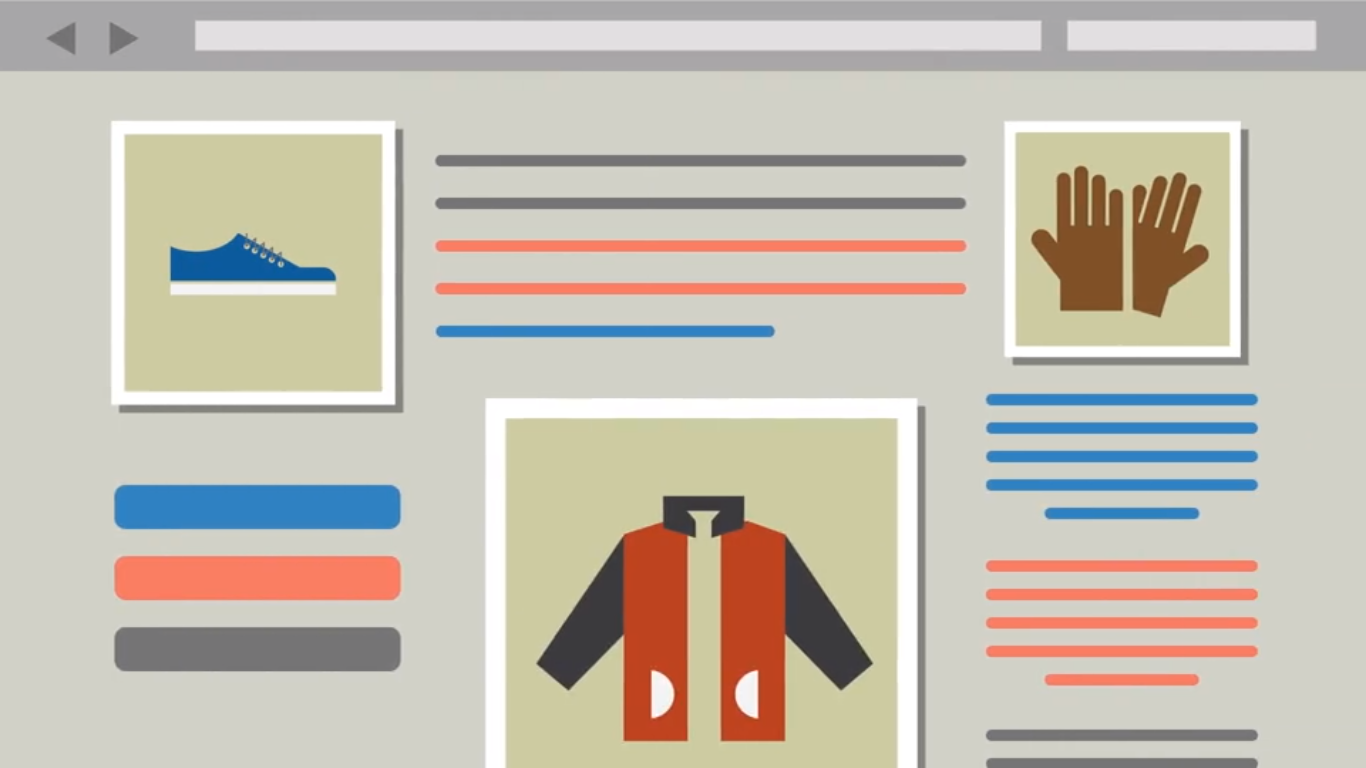
\includegraphics[width=10.5cm]{Resources/sort1.PNG}
	}
	\hspace{0mm}
	\subfloat[‌تبدیل محتوا به کارت‌های قابل مرتب‌سازی توسط کاربران و محول‌ کردن دسته‌بندی و مرتب‌سازی به کاربران سامانه به منظور تست و کشف الگوهای فکری کاربران‌]{
		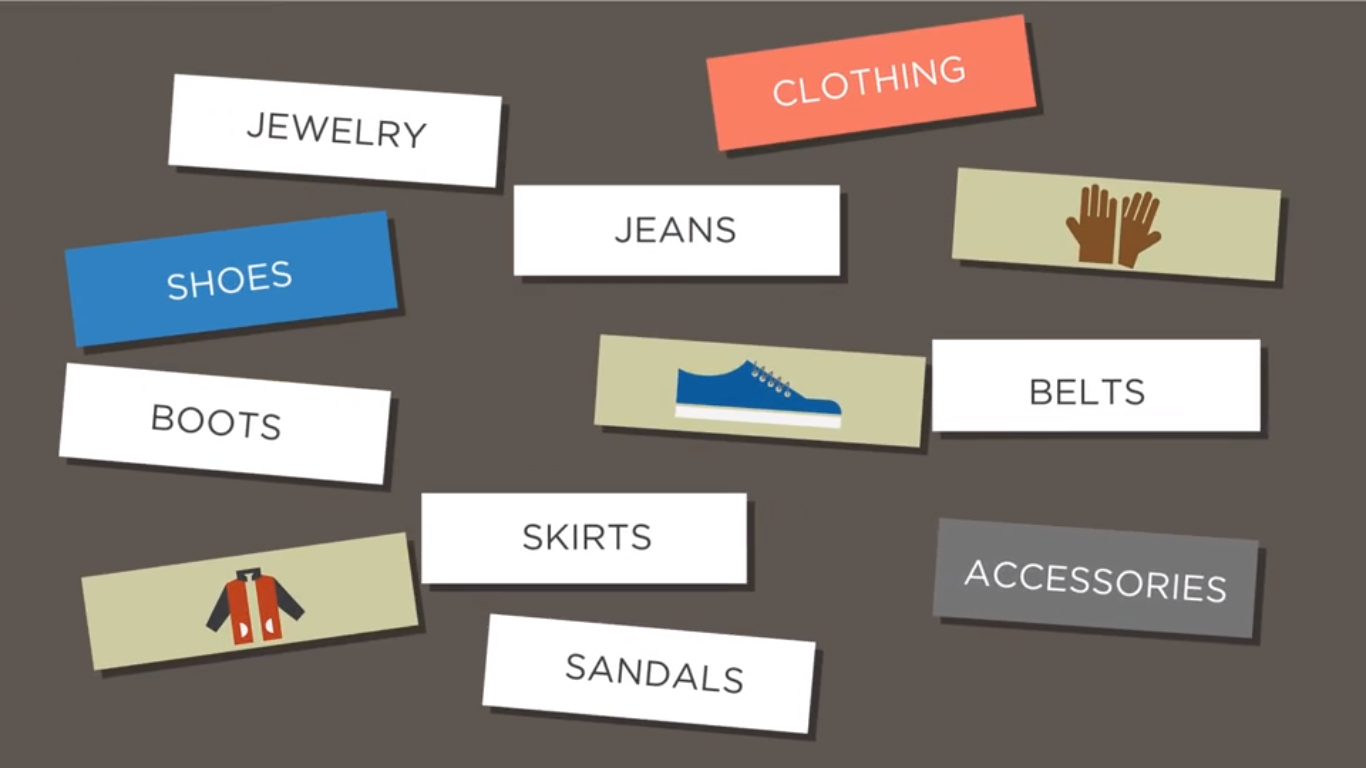
\includegraphics[width=10.5cm]{Resources/sort2.PNG}
	}
	\hspace{0mm}
	\subfloat[‌استفاده از الگوها و داده‌های استخراج شده از پاسخ کاربران در مرتب‌سازی کارت‌ها و نهایتا بهینه کردن ظاهر واسط کاربری‌]{
		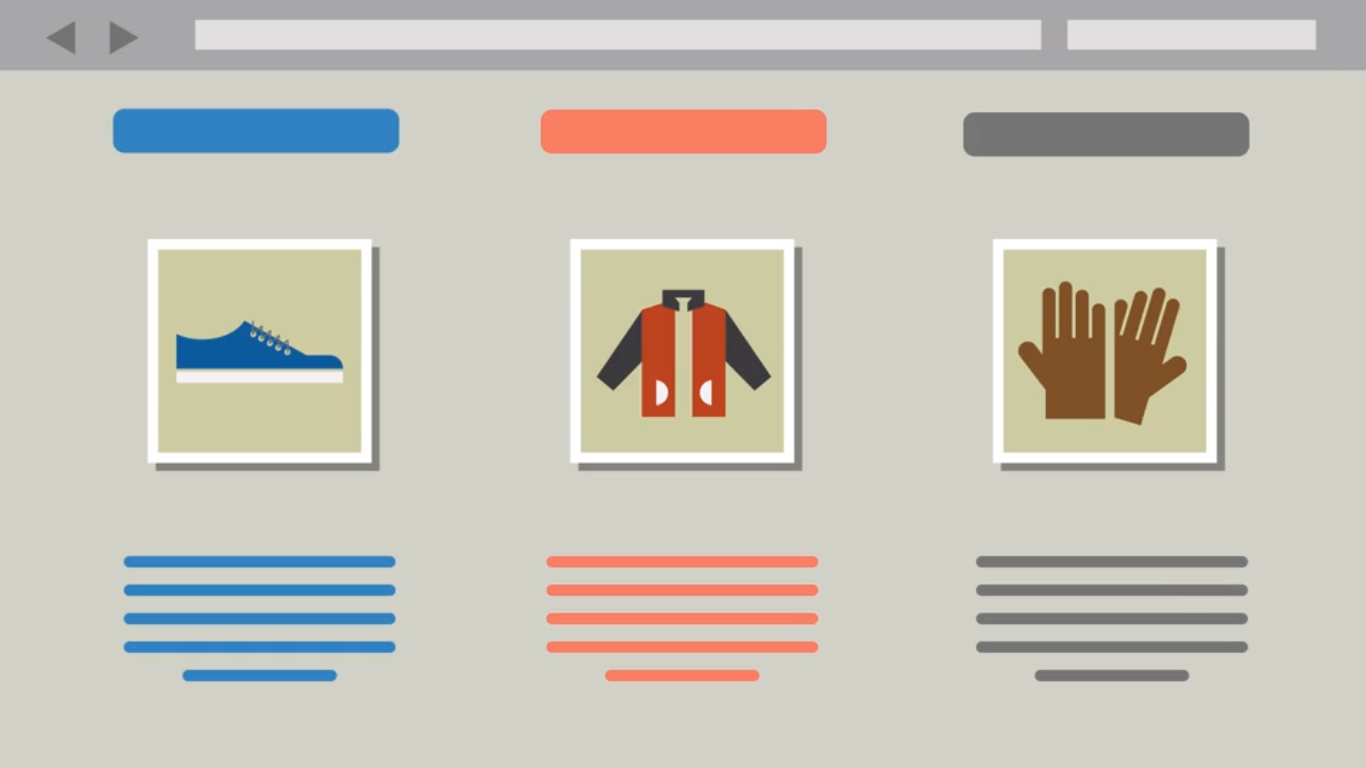
\includegraphics[width=10.5cm]{Resources/sort3.PNG}
	}
	\caption[تاثیر تست‌ها و الگوهای مرتب‌سازی در استفاده‌پذیری]
	{تاثیر تست‌ها و الگوهای مرتب‌سازی در استفاده‌پذیری
		\cite{noauthor_card_nodate}؛
		به منظور به دست آوردن داده‌های مرتب‌سازی، می‌بایست محتوای مورد نظر (آ) را در قالب کارت‌هایی درآورد  و سپس از شرکت‌کنندگان خواست که هرگونه که متمایل‌اند به مرتب‌سازی و دسته‌بندی این داده‌ها بپردازند. از پاسخ‌های برآمده از شرکت‌کنندگان می‌توان الگوهایی را استخراج کرد که بهینه‌ترین حالت چینش محتوا، از نظر کاربران، در رابط کاربری را می‌تواند نشان دهد (ج).
	}
	\label{fig:sorting}
\end{figure}
\section{روش‌های سنجش استفاده‌پذیری}
\begin{table}[H]
	\caption[بحث در مورد نحوه انجام مطالعه استفاده‌پذیری با توجه به روش‌های مختلف مطالعه]{
		بحث در مورد نحوه انجام مطالعه استفاده‌پذیری با توجه به روش‌های مختلف مطالعه
		\cite{albert_measuring_2013}
	}
	\label{tab:studies}
	\centering
	%	\resizebox{\textwidth}{!}{%
	\begin{tabular}{|C{5cm}|C{5cm}|}
		\hline
		\cellcolor{gray!25}
		‏ابتدا مطالعه آزمایشگاهی و سپس انجام مطالعه برخط
		&
		\cellcolor{gray!25}
		ابتدا مطالعه برخط و سپس مطالعه آزمایشگاهی	\\ \hline
		مشکلات ساده و کوچک را پیدا کرده یا حل می‌کنیم و بقیه مسائل و بحث‌ها به نمونه‌هایی با اندازه بزرگ‌تر سپرده می‌شود & ابتدا بزرگترین و اصلی‌ترین مشکلات را با داده‌های به دست آمده از مطالعه برخط، شناسایی می‌کنیم و سپس از مطالعات آزمایشگاهی استفاده می‌کنیم تا دانش کیفی بیشتری در مورد این مشکلات و مسائل به دست آوریم  \\ \hline
		راه‌حل‌ها، ایده‌ها و طرح‌های جدید با استفاده از تست آزمایشگاهی تولید می‌شوند و سپس توسط مطالعه برخط، مورد ارزیابی، سنجش و درستی‌آزمایی واقع می‌شوند & مصاحبه‌ها، تصاویر ویدیویی و نقل‌قول‌های مستقیم زیادی باید از کاربران جمع شود تا بتوان راه‌حل‌های جدید مطرح کرد و سپس در آزمایشگاه و در فضایی کوچکتر، با آن راه‌حل‌ها مسئله را حل کرد \\ \hline
		بازخورد کاربران و نحوه تعامل آن‌ها به صورت حضوری مورد بررسی و ارزیابی قرار می‌گیرد &  باید تمامی خصیصه‌ها در مورد کیفیت طراحی مورد پرسش و نظرسنجی قرار گیرند و اگر نتیجه نهایی مثبت بود، نیازی به انجام مطالعه آزمایشگاهی نیست \\ \hline
	\end{tabular}%
	%	}
\end{table}
به لطف فناوری وب و شبکه، امروزه محدود به یک روش سنجش و ارزیابی نیستیم. همانطور که از بررسی منابعی همچون
\cite{agarwal_assessing_2002}،
\cite{albert_measuring_2013}،
\cite{krug_dont_2018} و
\cite{noauthor_measuringu:_2018}
برمی‌آید، می‌توان خصیصه‌ها و اندازه‌گیری‌های مربوط به آن‌ها را تقریبا از هر روشی که ارزیابی بعدی از این داده‌ها را تضمین کند، به دست آورد. جمله پیشین به این معنی است که در مطالعه، سنجش و ارزیابی استفاده‌پذیری، نه تنها محدود به مشاهدات و آزمایشات آزمایشگاهی\RTLfootnote{
	به منظور مطالعه بیشتر می‌توان به مرجع
	\cite{li_crowdsourced_2016}
	مراجعه نمود که مروری روی انگیزه‌ها، روش‌ها و چالش‌های جمع‌سپاری می‌کند و از جمع‌سپاری به عنوان یک راه جمع‌آوری داده برای انجام ارزیابی‌ها و سنجش‌های مختلف نام می برد؛ در این منبع همچنین به دفعات متعدد اثبات شده است که هزینه استفاده از جمع‌سپاری برای جمع‌آوری داده به مراتب از روش‌هایی همچون روش‌های آزمایشگاهی کمتر بوده و با استفاده از این روش می‌توان با صرف زمان و هزینه کمتر، به نتایج گسترده‌تری رسید.
}
(که به معنای تعداد کم شرکت‌کنندگان و صرف زمان و هزینه زیاد است) نیستیم، بلکه می‌توانیم از روش‌هایی همچون مطالعات برخط استفاده کرده و حجم زیادی از تفاسیر و تحلیل‌ها را در زمان کمی به دست آوریم\RTLfootnote{
نکته قابل تامل از این نتیجه‌گیری این است که سازمان‌ها، کسب‌وکارها و شبکه‌های اجتماعی می‌توانند از قدرت کاربران خود استفاده کنند تا برای جمع‌آوری داده راهی هموارتر، که به دنبال آن سودآوری بیشتر خواهد آمد، داشته باشند. این به این معناست که همین پروژه می‌تواند در صورت پیاده‌سازی تجاری توسط یک سازمان دارای کسب‌وکاری از نوع
«\lr{B2C (Business to Client)}»
یک منبع درآمد اضافی باشد؛ کسب‌وکارهای نوپا
(\lr{Startups})
و سریس‌های مبتنی بر وب جدید را در نظر بگیرید. همه این کسب‌وکارها که سرویس خود را با کمک سامانه‌های مبتنی بر وب ارائه می‌دهند، همگی مایل‌اند که با صرف حداقل هزینه، به بهترین محصول برای شروع کسب‌وکار خود برسند. سازمان ارائه‌دهنده سرویس سنجش استفاده‌پذیری برای کسب‌وکارهای نوپا می‌تواند با استفاده از کاربران خود و با بهره‌گیری از روش‌های جمع‌سپاری و خرد‌کردن تست‌ها به میکرووظایف، داده‌های مربوط برای تست و سنجش استفاده‌پذیری محصولات نرم‌افزاری کسب‌وکارهای نوپا را فراهم کند. بنابراین این پروژه می‌تواند به عنوان یک طرح کسب‌وکاری
(\lr{Business Plan})
اولیه برای سازمان‌های درگیر با کاربران نهایی
(\lr{B2C})
و همچنین کسب‌وکارها
(\lr{B2B - Business to Business})
باشد.
}.\\
مطالعات برخط می‌توانند هم برای جمع‌آوری داده‌های کیفی و هم برای جمع‌آوری داده‌های کمی استفاده شوند؛ از طرفی دیگر در این نوع مطالعات می‌توان هم روی نگرش و هم روی رفتار شرکت‌کنندگان تامل کرد. به گفته مراجعی همچون
\cite{walker_high-fidelity_2002}
برخی از پژوهشگرانِ استفاده‌پذیری، ایده نوعی مطالعه ترکیبی را مطرح می‌کنند که در ادامه می‌توان به مطالعه برخط نیز آن را تعمیم داد. با در نظر گرفتن ایده‌های مختلفی، مرجع
\cite{albert_measuring_2013}
بررسی جامعی در مورد چگونگی مطالعه استفاده‌پذیری و در نهایت سنجش استفاده‌پذیری و جمع‌آوری داده و تحلیل آن‌ها انجام داده است که در جدول
\ref{tab:studies}
قابل مشاهده است.در این جدول یک نگاه کلی به دو روش شده است که الزاما نمی‌توان گفت کدام‌یک بهتر است\RTLfootnote{
	چرا که این مورد بسته به کاربرد بوده و در جایی که مثلا حل کردن مشکلات کوچک اهمیت زیادی دارد، می‌بایست در ابتدا مطالعه آزمایشگاهی و در مقیاس کوچک انجام دهیم؛ در موقعیتی هم که یافتن مسائل اصلی از اهمیت بالایی برخوردار است، می‌بایست از مطالعه برخط و سپس مطالعه آزمایشگاهی (به منظور ارائه راه‌حل) استفاده کنیم.
}؛ اما نکته حائز اهمیت این است که هر دو روش مطالعات برخط و آزمایشگاهی نقاط ضعف و قوت خود را دارند که می‌بایست در انجام مطالعات استفاده‌پذیری، این موارد و اینکه چگونه می‌توان از ترکیب هر دو نوع مطالعه بیشترین بازدهی را کسب کرد، در نظر گرفت. \\
در انجام مطالعه استفاده‌پذیری، 
بدیهی است که انجام مطالعه برخط، در صورت بهره‌ور نبودن، هزینه و زمان بسیاری را خواهد طلبید. همانطور که در بخش مقدمه مطرح شد، یکی از راه‌های کم‌هزینه برای جمع‌آوری داده زیاد با صرف هزینه کم و از طرفی بسیار قابل اطمینان
\cite{li_crowdsourced_2016}
، جمع‌سپاری است که در ساخت این ابزار نیز به عنوان یک روش اصلی برای مطالعه استفاده‌پذیری و پیدا کردن مشکلات اصلی استفاده‌پذیری در نظر گرفته شده است.
\section{ابزارهای مطالعه استفاده‌پذیری}
با بررسی‌های انجام شده از مهرماه سال ۱۳۹۶ تا زمان نگارش این اثر، بیش از ۸۰ ابزار، روش و تکنیک مطالعه و سنجش استفاده‌پذیری مورد بررسی موشکافانه قرار گرفتند که خلاصه این بررسی در جدول
\ref{tab:tools}
(رجوع شود به
\hyperref[sec:appendix]{پیوست})
قابل مشاهده است. لیست این ابزارها با مطالعه منابع برخط موجود و همچنین با فعالیت چند ساله نگارنده در حوزه توسعه سامانه‌های مبتنی بر وب متن‌باز و استفاده از منابع آکادمیک موجود تهیه شده است. با جمع‌آوری داده در مورد این ابزارها، شروع به بررسی نحوه سازوکار آن‌ها کردیم. در مورد برخی از این ابزارها که رایگان و یا متن‌باز بودند، بررسی و استفاده آن‌ها کار آسانی بود و با چندین نمونه آزمایشی توانستیم ویژگی‌های اصلی ابزار را شناسایی کنیم؛ در مورد قسمت دیگر ابزارها که به تمامی پولی بودند و یا استفاده از قسمتی از آن‌ها مستلزم پرداخت هزینه بود (نیمه رایگان)\RTLfootnote{
	اصطلاحا به این نوع استفاده،
«\lr{Freemium}»
	گفته می‌شود که ترکیبی از دو لغت
«\lr{Premium}»
	و
«\lr{Free}»
	می‌باشد. در این حالت معمولا قسمتی از سرویس - که برای شروع به کار و یا استفاده اولیه می‌باشد - به صورت مجانی در دسترس بوده ولی مصرف‌کننده برای استفاده از ویژگی‌های دیگر ابزار می‌بایست هزینه خاصی را بپردازد و یا اشتراک خریداری کند.
}،
با استفاده از نقد و بررسی‌های موجود در سطح جوامع برخط و انجمن‌های گفتگو و همچنین دموها و اطلاعات موجود در وبسایت ابزارها که توسط سازندگان در دسترس عموم قرار گرفته بود، اطلاعات مربوط به نحوه کار و استفاده با ابزار را استخراج کردیم که در نهایت تمامی ابزارها را از لحاظ سناریوهای قابل انجام، بررسی نمودیم. شایان ذکر است که تعداد بسیار اندکی از ابزارهای مطرح (فقط یک ابزار که روی ردیابی چشم کاربر تاکید دارد) بر آزمایش‌های کوچک بسنده می‌کند و از جمع‌سپاری استفاده نمی‌کند؛ همچنین گفتنی است که هرکدام از این ابزارها، یا از سکوهای جمع‌سپاری\LTRfootnote{
	Crowdsourcing Platforms
} به منظور انجام جمع‌سپاری استفاده می‌کنند و یا خودشان با استفاده از قراردادهای داخلی، پلتفرم‌های خصوصی و یا سایر امکانات درون سازمانی خودشان، برای جمع‌آوری داده از روش جمع‌سپاری اقدامات لازم را انجام می‌دهند.\\
پیش‌تر ده سناریوی مهم برای بررسی و مطالعه استفاده‌پذیری مطرح شد که در جدول
\ref{tab:tools}،
در یک سو این سناریوها قابل مشاهده‌اند و در سویی دیگر ابزارها لیست شده‌اند. به منظور خلاصه‌سازی نتایج حاصل از این مطالعه، هرکدام از این ابزارها را برحسب نحوه کارکردشان و هدف نهایی هر کدام، در دسته‌هایی قرار می‌دهیم که الزاما هم از یکدیگر جدا نیستند؛ به عبارت دیگر، یک ابزار می‌تواند در دو یا چند دسته نیز قرار بگیرد.\\
\begin{longtable}[c]{|C{3cm}|C{3.2cm}|C{3.2cm}|C{3.2cm}|C{0.8cm}|}
		\caption[دسته‌بندی ابزارهای مطرح در این پژوهش برای مطالعه استفاده‌پذیری]{
		دسته‌بندی ابزارهای در این پژوهش برای مطالعه استفاده‌پذیری؛ ابزارها مطابق با هدفی که هرکدام دنبال می‌کنند و نیز کارکردی که برای مصرف‌کنندگان دارند، در دسته‌هایی، که الزاما از یکدیگر انحصار ندارند، قرار گرفته‌اند.
	}
	\label{tab:tools_category} \\
		\hline
		\multicolumn{5}{| c |}{دسته‌بندی ابزارهای مطرح در این پژوهش برای مطالعه استفاده‌پذیری}\\
		\hline
		کارکرد و هدف نهایی & ورودی & نحوه کار & خروجی & تعداد ابزارها \\
		\hline
		\endfirsthead
		
		\hline
		\multicolumn{5}{| c |}{ادامه جدول \ref{tab:tools_category}}\\
		\hline
		کارکرد و هدف نهایی & ورودی & نحوه کار & خروجی & تعداد ابزارها \\
		\hline
		\endhead
		\multicolumn{5}{| c |}{ادامه جدول در صفحه بعد...}\\
		\hline
		\endfoot
		
		\hline
		\endlastfoot
		انتخابگر میان دو یا چند طرح & دو یا چندین طرح مفهومی/پیاده‌سازی‌شده مختلف & نمایش انتخاب‌های موجود به کاربر و دریافت پاسخ از وی و تجمیع داده‌ها & داده‌های تجمیع شده و نتیجه نهایی ترجیحات کاربران & 6 \\ \hline
		تحلیل‌گر & نقطه دسترسی به کل یا بخشی از سامانه & جمع‌آوری داده از روی پروفایل کاربران، تاریخچه کلیک‌ها، میزان وقت صرف شده در هر صفحه، موقعیت جغرافیایی و ... & تحلیل‌های پیشرفته از رفتار کاربران & 15 \\ \hline
		سنجش‌گر سازگاری با محیط‌های مختلف & نقطه دسترسی به کل یا بخشی از سامانه & بررسی نحوه رفتار سامانه  روی مرورگرها و سامانه‌های کاربری مختلف & مقدار سازگاری سامانه/صفحه مورد نظر با تغییرات محیطی & 4 \\ \hline
		ردیابی‌کننده  چشم کاربر & محیط آزمایشگاهی و کاربر مورد نظر برای تست & بررسی رفتار کاربر به واسطه حرکات چشم او & عملکرد رفتار کاربر در مواجهه با سامانه & 1 \\ \hline
		تولیدکننده نقشه حرارتی & نقطه دسترسی به کل یا بخشی از سامانه & جمع‌‌آوری داده‌های مربوط به کلیک‌های کاربران & نقشه‌های حرارتی که نشان‌دهنده نقاط با میزان توجه‌های متفاوت توسط کاربران است & 22 \\ \hline
		سنجش‌‌گر سرعت بارگزاری & نقطه دسترسی به کل یا بخشی از سامانه & دسترسی به سامانه در محیط‌ها و شرایط مختلف & کارایی و نحوه پاسخگویی سامانه & 5 \\ \hline
		پرسشنامه‌ساز & سوالات، موارد دارای ابهام و نظرسنجی‌های کیفیتی مطرح & پرسش از کاربران و شرکت‌کنندگان در نظرسنجی & پاسخ‌های تجمیع‌شده و تحلیلی از پاسخ‌های کاربران & 8 \\ \hline
		سنجش‌گر نمونه‌های مفهومی & نمونه‌های مفهومی و طرح‌های اولیه سامانه & طرح سوال از کاربران و درخواست انجام عملیات مشخص روی آن‌ها & نتایج تجمیع‌شده از میزان رضایت کاربران از طرح‌های اولیه و مفهومی & 20 \\ \hline
		سنجش‌گر کارایی کاربر & نقطه دسترسی به کل یا بخشی از سامانه & طرح پرسش‌هایی به منظور شروع تعامل کاربر و جمع‌آوری پاسخ کاربران & نتایج کارایی کاربران در تعامل با سامانه & 25 \\ \hline
		ثبت‌کننده عملیات کاربر & نقطه دسترسی به کل یا بخشی از سامانه & ردیابی حرکات کاربر و تعاملات وی با سامانه & نتایج تحلیل‌شده رفتار کاربر در تعامل با سامانه & 16 \\ \hline
		اعلام‌کننده بازخورد کاربر & نقطه دسترسی به کل یا بخشی از سامانه & طرح پرسش‌هایی به منظور شروع تعامل کاربر و جمع‌آوری پاسخ کاربران & تحلیل احساسات نهایی و امتیازات کاربر به سامانه & 7 \\ \hline
\end{longtable}
مطابق جدول
\ref{tab:tools_category}
و البته شکل
\ref{fig:category_tools}
مشاهده می‌شود که بیشترین تمرکز در بین ابزارها، روی سنجش کارایی کاربران است که برای همین منظور، از تولید نقشه‌های حرارتی\LTRfootnote{Heatmaps} بهره برده می‌شود.\\
همچنین ملاحظه می‌شود که پس از موارد ذکر شده، سنجش و تست نمونه‌های مفهومی، از جمله هدف‌های محبوب ابزارها بوده است؛ البته با توجه به موارد ذکر شده در فصول پیشین و توجه به این نکته که افزایش استفاده‌پذیری طرح‌های مفهومی و اولیه، باعث کاهش هزینه‌ها و همچنین افزایش رضایت کاربری خواهد شد، می‌توانستیم از ابتدا نیز پیش‌بینی کنیم که رفع نواقص نمونه‌ها و طرح‌های اولیه از اهداف مهم ابزارها می‌باشد.\\

حال با شناخت اهداف هر کدام از این ابزارها، بد نیست به نحوه اندازه‌گیری خصیصه‌های کیفیتی مرتبط با استفاده‌پذیری در هر کدام بپردازیم. با بررسی این ۸۳ ابزار و با تجمیع داده‌های موجود در جدول
\ref{tab:tools}
می‌توان به یک سری الگوی تکراری در روش‌های اندازه‌گیری رسید که به طور کاملا مجزا و در ابزارهای متفاوتی دیده‌ می‌شوند. به منظور جمع‌آوری این الگو‌ها و بحث در مورد هر کدام، به بررسی موردی هرکدام از ابزارها پرداختیم؛ در این بررسی، سوال اصلی این بود که ابزار مورد نظر چگونه برای رسیدن به هدف مورد نظر و ماموریت خاص خود، به سنجش و اندازه‌گیری خصیصه‌های کیفیتی مرتبط با استفاده‌پذیری می‌پردازد؟\\
با استفاده از داده‌هایی که از ابزارهای مختلف داشتیم، سعی در نام‌گذاری برای هر الگوی مورد استفاده توسط گروهی از ابزارها کردیم. با در نظر گرفتن هدف هر ابزار و همچنین پاسخ دادن به سوال فوق در مورد هر ابزار، به نتایج بسیار جالبی رسیدیم که خلاصه آن‌ها در جدول
\ref{tab:scenario_measurement}
بیان شده است.
\begin{figure}[H]
	\centering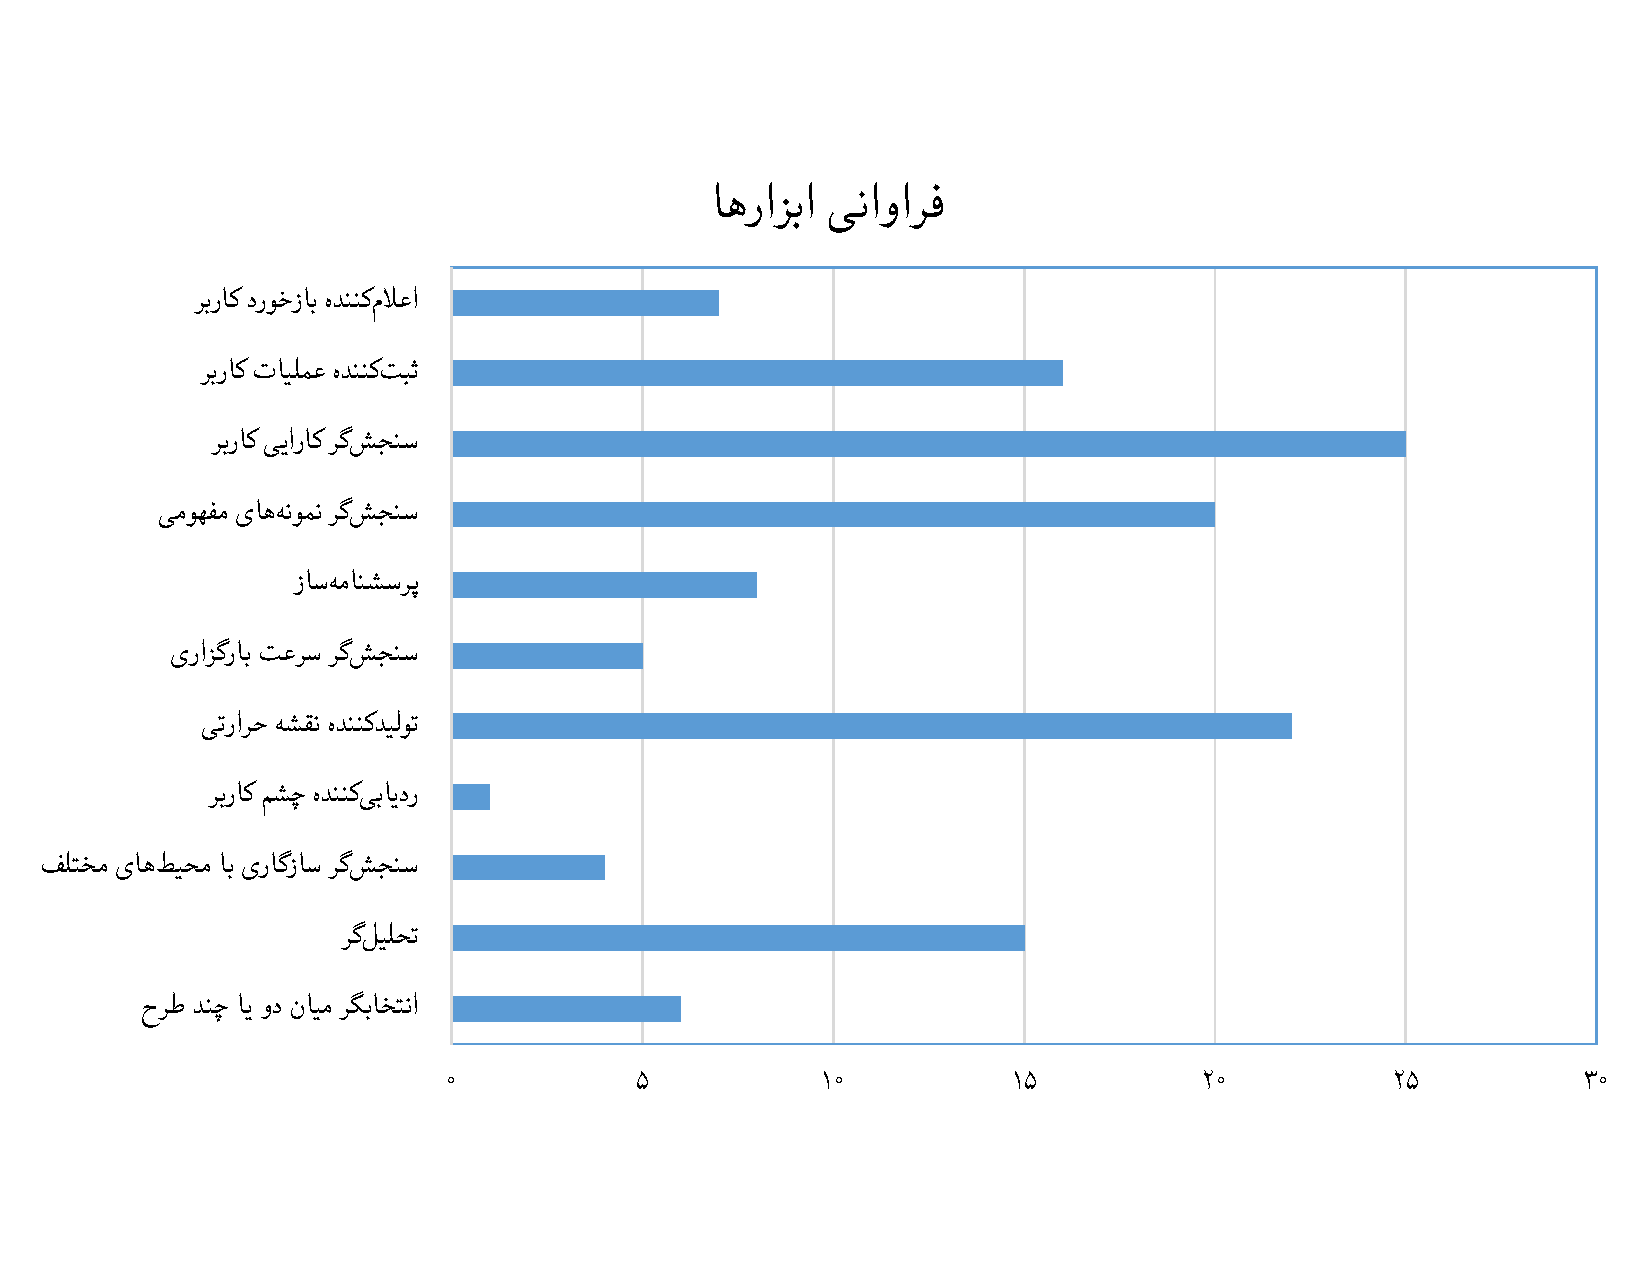
\includegraphics[width=0.8\linewidth]{Resources/tools_category.pdf}
	\caption[فراوانی ابزارهای موجود در هر دسته مطرح]
	{فراوانی ابزارهای موجود در هر دسته مطرح
	}
	\label{fig:category_tools}
\end{figure}
	\begin{longtable}[c]{|C{7cm}|C{6cm}|C{1.2cm}|}
			\caption[
		فراوانی ابزارهای بررسی شده و الگوهای مورد استفاده توسط هرکدام
		]{
			فراوانی ابزارهای بررسی شده و الگوهای مورد استفاده توسط هرکدام؛
		}
		\label{tab:scenario_measurement} \\
				\hline
		\multicolumn{3}{| c |}{فراوانی ابزارهای بررسی شده و الگوهای مورد استفاده توسط هرکدام}\\
		\hline
		سناریوی مطرح & روش سنجش و اندازه‌گیری & فراوانی ابزارها \\
		\hline
		\endfirsthead
		
		\hline
		\multicolumn{3}{| c |}{ادامه جدول \ref{tab:scenario_measurement}}\\
		\hline
		سناریوی مطرح & روش سنجش و اندازه‌گیری & فراوانی ابزارها \\
		\hline
		\endhead
		\multicolumn{3}{| c |}{ادامه جدول در صفحه بعد...}\\
		\hline
		\endfoot
		\multicolumn{3}{| c |}{انتهای جدول}\\
		\hline
		\endlastfoot
		\multirow{3}{*}{انجام یک تراکنش} & پرسشنامه متنی و تصویری & 7 \\ \cline{2-3} 
		& تست پیمایشی & 3 \\ \cline{2-3} 
		& ذخیره‌سازی کلیک‌های کاربران و پروفایل‌سازی & 14 \\ \hline
		\multirow{3}{*}{مقایسه محصولات} & تست ترجیح & 10 \\ \cline{2-3} 
		& تست‌های مرتبط با حافظه کوتاه‌مدت & 6 \\ \cline{2-3} 
		& پرسشنامه متنی و تصویری & 13 \\ \hline
		\multirow{3}{*}{ارزیابی استفاده مکرر از محصول} & ذخیره‌سازی کلیک‌های کاربران و پروفایل‌سازی & 6 \\ \cline{2-3} 
		& تست‌های مرتبط با حافظه کوتاه‌مدت & 6 \\ \cline{2-3} 
		& تست پیمایشی & 7 \\ \hline
		\multirow{4}{*}{ارزیابی پیمایش و معماری اطلاعات سامانه} & پرسشنامه متنی و تصویری & 9 \\ \cline{2-3} 
		& تست پیمایشی & 14 \\ \cline{2-3} 
		& استفاده از حسگر ردیاب چشم & 1 \\ \cline{2-3} 
		& ذخیره‌سازی کلیک‌های کاربران و پروفایل‌سازی & 8 \\ \hline
		\multirow{2}{*}{افزایش آگاهی} & پرسش سوالات مربوط به طرح‌های مفهومی & 7 \\ \cline{2-3} 
		& تست ترجیح & 5 \\ \hline
		\multirow{5}{*}{کشف مشکل} & بررسی فنی و جزئیات کد & 6 \\ \cline{2-3} 
		& ذخیره‌سازی کلیک‌های کاربران و پروفایل‌سازی & 9 \\ \cline{2-3} 
		& پرسش سوالات مربوط به طرح‌های مفهومی & 9 \\ \cline{2-3} 
		& استفاده از حسگر ردیاب چشم & 1 \\ \cline{2-3} 
		& پرسشنامه متنی و تصویری & 11 \\ \hline
		\multirow{3}{*}{حداکثرسازی استفاده‌پذیری یک محصول حیاتی} & استفاده از حسگر ردیاب چشم & 1 \\ \cline{2-3} 
		& تست ترجیح & 8 \\ \cline{2-3} 
		& ذخیره‌سازی کلیک‌های کاربران و پروفایل‌سازی & 4 \\ \hline
		\multirow{4}{*}{ایجاد تجربه کاربری مثبت} & پرسشنامه متنی و تصویری & 3 \\ \cline{2-3} 
		& تست ترجیح & 8 \\ \cline{2-3} 
		& پرسش سوالات مربوط به طرح‌های مفهومی & 7 \\ \cline{2-3} 
		& ذخیره‌سازی کلیک‌های کاربران و پروفایل‌سازی & 6 \\ \hline
		\multirow{6}{*}{ارزیابی تاثیرات تغییرات جزئی و نامحسوس} & بررسی فنی و جزئیات کد & 3 \\ \cline{2-3} 
		& استفاده از حسگر ردیاب چشم & 1 \\ \cline{2-3} 
		& تست ترجیح & 5 \\ \cline{2-3} 
		& ذخیره‌سازی کلیک‌های کاربران و پروفایل‌سازی & 9 \\ \cline{2-3} 
		& پرسشنامه متنی و تصویری & 7 \\ \cline{2-3} 
		& تست‌های مرتبط با حافظه کوتاه‌مدت & 6 \\ \hline
		\multirow{3}{*}{مقایسه طراحی‌های مختلف} & تست ترجیح & 10 \\ \cline{2-3} 
		& پرسش سوالات مربوط به طرح‌های مفهومی & 7 \\ \cline{2-3} 
		& پرسشنامه متنی و تصویری & 9 \\ \hline
\end{longtable}
با استفاده از تجمیع داده‌های جدول ملاحظه می‌شود که به منظور انجام یکی از ده سناریوی مطرح در مطالعه استفاده‌پذیری، این ابزارها از الگوهای مشترک و مشخصی استفاده می‌کنند که می‌توان آن‌ها را در دسته‌های یکسان قرار داد.شایان ذکر است که طبق جدول
\ref{tab:tools_category}،
یک ابزار می‌تواند بیش از یک هدف و سناریو را مدنظر قرار دهد، به همین منظور دسته‌بندی این جدول، به طور کامل فضای ابزارهای مورد بررسی را افراز نمی‌کند و در نتیجه ابزارهایی را می‌توان یافت که از چندین الگو برای انجام یک یا چندین سناریو استفاده می‌کنند.\\
با مطالعه ابزارها و روش‌های موجود، الگوهای مشابهی از اعمال و راه‌حل‌ها برای حل مسائل مشاهده می‌شوند. مطابق جدول
\ref{tab:scenario_measurement}
هشت الگوی تکراری به منظور سنجش استفاده‌پذیری در این ابزارها دیده می‌شود که عبارتند از:
\begin{enumerate}
	\item
	پرسشنامه متنی و تصویری: در رابطه با یک یا چند تصویر مرتبط با یک طرح مفهومی یا نتیجه حاصل از یک کد، سوالاتی که اغلب پاسخ چند گزینه‌ای داشته، ولی می‌توانند پاسخ‌های کوتاه و بلند نیز داشته باشند، پرسیده می‌شود. در صورتی که پاسخ‌هایی غیر از چندگزینه‌ای از کاربران خواسته شود، می‌بایست پردازش‌های دیگری به منظور تحلیل دادگان آن‌ها انجام شود. البته باید توجه داشت که گاهی حتی سوالات به صورت تمام متنی هم هستند و ممکن است تصویری در پرسشنامه نباشد.
	\item 
	تست پیمایشی: با استفاده از طرح‌های مفهومی و یا صفحات اچ‌تی‌ام‌ال پیاده‌سازی شده، درخواست انجام یک یا چند عمل مشخص از کاربر می‌شود و پاسخ‌های وی با در نظر گرفتن زمان پاسخ ثبت می‌شوند.
	\item 
	ذخیره‌سازی کلیک‌های کاربران و پروفایل‌سازی: تمام تعاملات کاربر که از طریق دستگاه ورودی ماوس و حتی گاها کیبرد هستند، با رعایت ترتیب زمانی و زمان رخ‌داد، ذخیره شده و مورد بررسی و تحلیل واقع می‌شوند.
	\item 
	تست ترجیح: دو یا چند نمونه از طرح‌های اولیه و یا رابط‌های پیاده‌سازی شده به کاربر نمایش داده می‌شوند و از وی در مورد ترجیحاتش سوال پرسیده می‌شود.
	\item 
	تست‌های مرتبط با حافظه کوتاه مدت: به مدت محدودی، قسمتی از محتوا و یا واسط کاربری، مورد نمایش قرار می‌گیرد و پس از اتمام مهلت نمایش، از کاربر سوالاتی پرسیده می‌شود.
	\item 
	استفاده از حسگر ردیاب چشم:	این الگو که نوعی پروفایل‌سازی از کاربر است، با استفاده از تجهیزات اختصاصی و به منظور بررسی موشکافانه رفتار کاربر در تعامل با سیستم، انجام می‌شود. در نهایت از حسگر نیز به عنوان یک دستگاه ورودی استفاده شده است و تفاوت چندانی با حالت ذخیره‌سازی تعاملات با ماوس و کیبرد ندارد جز اینکه، جزئیات در اینجا بیشتر مورد توجه هستند.
	\item 
	پرسش سوالات مربوط به طرح‌های مفهومی: به طور خاص در مورد طرح‌های اولیه و خام و مفهومی که هنوز پیاده‌سازی نشده‌اند، سوالاتی از شرکت‌کننده پرسیده می‌شود.
	\item 
	بررسی فنی و جزئیات کد: در این الگو، به طور خاص، روی کد تولید شده تمرکز می‌شود و ابزار، اغلب به صورت اتوماتیک و صرفا با دریافت برخی از تنظیمات توسط کاربر، به بررسی جزئیات کد می‌پردازد. تمرکز اصلی در اینجا کشف خطاهای ناخواسته و غیرقابل تشخیص توسط انسان است که می‌تواند نقش شگرفی در افزایش استفاده‌پذیری بازی کند.
\end{enumerate}
با توجه به اطلاعات موجود در فصل‌های گذشته و با بررسی ابزارها، رویکردها و تکنیک‌های موجود در مطالعه استفاده‌پذیری، می‌توان گفت که هر ده سناریوی مطرح در مطالعه استفاده‌پذیری، از اهمیت خاصی برخوردارند که نمی‌توان منکر آن بود و در افزایش استفاده‌پذیری یک محصول، فارغ از ویژگی‌های تجاری محصول، تمامی سناریوها می‌بایست مورد نظر باشند. بنابراین با استفاده از مدل معرفی شده در منبع
\cite{albert_measuring_2013}
می‌بایست برای تمامی خصیصه‌های عنوان شده، یک یا چند روش اندازه‌گیری و یا زیرخصیصه مطرح کنیم که بتوانیم به پیاده‌سازی ابزاری کارا و موثر در مطالعه استفاده‌پذیری، بپردازیم. در فصل بعد به این مهم و همچنین ویژگی‌های ابزار هدف پرداخته‌ایم.
\section{راستی آزمایی مطالعات جمع‌سپاری}
توجه به این نکته حائز اهمیت است که راستی آزمایی و همچنین اثبات درستی ادعای کاربران شرکت کننده در مطالعات برخط، به خصوص هنگامی که بحث جمع‌سپاری در میان است، کار آسانی نبوده و از زمان مطرح شدن کاربردهای جمع‌سپاری، افزایش کیفیت محصول نهایی در روش‌های درگیر با جمع‌سپاری نیز، همواره مطرح بوده است
\cite{li_crowdsourced_2016}.
در سال‌های اخیر به طور خاص، حجم تحقیقاتی که به مطالعه و بررسی رفتار کاربران تولید کننده محتوای هرز\LTRfootnote{Spammer} و همچنین از بین بردن تاثیر این رفتارها و محتواها روی مطالعات مبتنی بر جمع‌سپاری، بیشتر شده است که شاید گل سرسبد این تحقیقات را می‌توان در یک بررسی کلی و جامع از سوی آقای لی و همکارانش در مرجع
\cite{li_crowdsourced_2016}
را شاهد هستیم؛ این پژوهش، تحقیقات انجام شده در راستای بهینه‌سازی فرآیندها و مطالعات مربوط به جمع‌سپاری تا سال ۲۰۱۶ را، در سه بعد کنترل کیفیت، کنترل هزینه و کنترل تاخیر دستیابی به نتیجه بررسی می‌کند و با بررسی بیش از صد کار پژوهشی برتر در زمینه روش‌های مرتبط با کنترل، مدیریت و افزایش کیفیت خروجی فرآیند جمع‌سپاری، چندین دسته رویکرد کلی مطرح می‌نماید:
\begin{enumerate}
	\item 
	مدل‌سازی کارگران\LTRfootnote{Worker Modeling} به منظور شناخت کیفیت کار هریک و قضاوت نتیجه از روی کیفیت کار هر کارگر و در صورت نیاز، حذف نتایج مربوط به کارگران با کیفیت کم،
	\item 
	حذف کارگران\LTRfootnote{Worker Elimination}  با کیفیت کم به منظور جلوگیری از بروز ابهام و یا افت کیفیت در خروجی نهایی جمع‌سپاری و کاهش راندمان سامانه،
	\item 
	تجمیع پاسخ‌ها\LTRfootnote{Answer Aggregation} و قضاوت از روی تفاوت پاسخ‌های هر کارگر به سوالات و شرایط مختلف،
	\item 
	تخصیص وظایف\LTRfootnote{Task Assignment} (کارگرهای) متناسب به یک کارگر به منظور حداکثر کردن کیفیت خروجی نهایی.
\end{enumerate}
بدیهی است که استفاده از هرکدام از رویکرد‌های فوق هزینه‌هایی به همراه دارد که از جمله آن هزینه‌ها می‌توان به پیچیدگی بیش‌ از حد در پیاده‌سازی اشاره کرد؛ البته ناگفته نماند که هرچقدر وسعت کار بیشتر شده و جوامع بزرگتری در جمع‌سپاری شرکت‌کنند، اهمیت کار کنترل کیفیت بیش از پیش خواهد شد و چه بسا که هزینه‌های زیاد کنترل کیفیت، به افزایش کیفیت خروجی آن بچربد؛ اما بد نیست به این نکته توجه کنیم که تمرکز اصلی این پروژه روی ساخت ابزاری برای افزایش استفاده‌پذیری است و نه ساخت یک سکوی جمع‌سپاری پیشرفته. بنابراین استفاده از رویکردهای پیچیده و هزینه‌بر در این پروژه، ممکن است سود چندانی در نهایت نداشته باشد.\\
از جمله روش‌های بسیار ساده‌ای که طبق مطالعات انجام شده در مرجع
\cite{li_crowdsourced_2016}،
در سال‌های اخیر به منظور جلوگیری از تاثیرگذاری محتوای هرز روی نتایج تجزیه و تحلیل داده‌های حاصل از جمع‌سپاری مطرح شده است، روش مدل‌سازی کارگران نامیده می‌شود. اساسا این رویکرد فرضیاتی را در نظر می‌گیرد که برای محقق استفاده کننده از جمع‌سپاری معلوم‌اند ولی برای کارگران نامعلوم؛ در نتیجه کارگران در مواجهه با مسائلی که از این فرضیات تغذیه می‌شوند، رفتاری از خود بروز می‌دهند و نتایجی را باقی می‌گذارند که محقق می‌تواند روی تاثیر یا عدم تاثیر آن رفتار یا بازخورد قضاوت کند و آستانه مشخصی روی کیفیت کارِ کارگران بگذارد. می‌توان ایده را به صورت ساده‌تر و به شرح مقابل توضیح داد: اگر کارگری در فرآیند جمع‌سپاری، به سوال یا درخواستی بسیار ساده و بدیهی (از دیدگاه محقق) واکنش و پاسخی نامتعارف و یا ناصحیح بدهد، کیفیت کار وی پایین شناخته شده و خروجی رفتار وی از جمله‌ کاندیداهای حذف در نتیجه‌گیری نهایی است.\\
طی این مدل‌سازی، به هر کدام از کاربران عددی بین یک تا صفر، تحت عنوان
$q$
تخصیص داده می‌شود که این عدد بیانگر تعداد پاسخ‌های درست کاربر به درخواست‌ها و سوالات است
\cite{li_crowdsourced_2016}.
به عبارت دیگر می‌توان گفت:
\begin{equation}
	q = Pr(p=t)
\end{equation}
که نماد $p$ در اینجا پاسخ کارگر به درخواست بوده و نماد $t$ بیانگر پاسخ درست درخواست است. مرجع
\cite{li_crowdsourced_2016}
همچنین مجددا یادآوری می‌کند که به دلیل  تک‌بعدی و احتمالاتی بودن $q$، برخی از پژوهش‌های پیشین سعی در دخیل کردن پارامترهای تاثیرگذار دیگری همچون سابقه کارگر و یا گسترده‌تر کردن محدوده $q$ و سایر رویکردها را به منظور افزایش هرچه بهتر این کیفیت دارند که مجددا باید خاطرنشان شد که به خاطر پیچیدگی زیاد، از ذکر جزییات صرف نظر می‌شود.\\
همانطور که مشخص است، فرض این رویکرد در وجود حقیقت محضی است که محقق (درخواست دهنده جمع‌سپاری) از آن مطلع است و معیار سنجش کار کارگران قرار می‌گیرد که البته میزان سختی انجام درخواست، با هدف تعیین کیفیت کارگران، کاملا بستگی به محقق دارد. در بعضی مطالعات ممکن است صرفا به جهت تشخیص دادن ربات از انسان و جلوگیری از تاثیرگذاری ربات‌ها روی مطالعه، این کار انجام شود و در بعضی دیگر، همانند برخی مطالعات استفاده‌پذیری، به منظور یافتن کاربران تولیدکننده هرزنامه.
\begin{table}[H]
	\caption[رتبه بندی روش‌های مطرح برای کنترل کیفیت جمع‌سپاری]{
		رتبه بندی روش‌های مطرح برای کنترل کیفیت جمع‌سپاری؛ با توجه به اطلاعات به دست آمده از دانش زمینه، می‌توان روش‌های مطرح را از نظر کم‌هزینه بودن و سادگی رتبه‌بندی کرد. بر این اساس آسان‌ترین راه‌حل برای کنترل کیفیت مطالعات جمع‌سپاری، استفاده از رویکرد مدل‌سازی کارگران است اما باید توجه داشت که این رویکرد الزاما به معنی بهترین نتیجه نخواهد بود. همچنین توجه شود که طبق مرجع ذکر شده، مقایسه کیفیت کار خروجی به عوامل بسیار زیادی بستگی دارد و نمی‌توان در برابر همچون پیچیدگی، آن را مقایسه کرد.
	}
	\label{tab:crowdquality}
	\centering\begin{tabular}{|C{4cm}|C{7cm}|C{1cm}|}
		\hline
		رویکرد & شرط لازم برای انجام & رتبه در پیاده‌سازی آسان\\ \hline
		مدل‌سازی کارگران & داشتن درخواست‌هایی با پاسخ مشخص & ۱ \\ \hline
		حذف کارگران کم‌کیفیت & دخیل‌کردن پارامترهای دیگر در مدل‌سازی کارگران از جمله پیشینه تاریخی وی & ۲ \\ \hline
		تجمیع پاسخ‌ها و در نظر گرفتن تفاوت‌های کارگران & به کار بردن استراتژی رای‌گیری در انجام وظایف & ۳ \\ \hline
		تخصیص وظایف منحصر به فرد به هر کارگر & شناسایی ویژگی‌های هر کارگر (درخواست) و تناظر آن با درخواست (کارگر) متناسب با آن & ۴ \\ \hline
	\end{tabular}
\end{table}
چکیده‌ای از بحث‌های مطرح شده در مورد مدیریت کیفیت خروجی فرآیند جمع‌سپاری را می‌توان در جدول
\ref{tab:crowdquality}
مشاهده کرد؛ طبق این طبقه‌بندی، برای کاربردهای کوچک و مطالعاتیٍ نه چندان بزرگ، استفاده از رویکردهای ساده‌تر و کم‌هزینه‌تر می‌تواند به عنوان هیوریستیکی برای کم کردن هزینه‌های ناشی از پیاده‌سازی باشد؛ پیاده‌سازی‌هایی همچون این پروژه که تمرکز اصلیشان چیزی غیر از جمع‌سپاری است و از جمع‌سپاری به عنوان راهکاری برای حل مسئله خود استفاده می‌کنند.




